% The document class supplies options to control rendering of some standard
% features in the result.  The goal is for uniform style, so some attention 
% to detail is *vital* with all fields.  Each field (i.e., text inside the
% curly braces below, so the MEng text inside {MEng} for instance) should 
% take into account the following:
%
% - author name       should be formatted as "FirstName LastName"
%   (not "Initial LastName" for example),
% - supervisor name   should be formatted as "Title FirstName LastName"
%   (where Title is "Dr." or "Prof." for example),
% - degree programme  should be "BSc", "MEng", "MSci", "MSc" or "PhD",
% - dissertation title should be correctly capitalised (plus you can have
%   an optional sub-title if appropriate, or leave this field blank),
% - dissertation type should be formatted as one of the following:
%   * for the MEng degree programme either "enterprise" or "research" to
%     reflect the stream,
%   * for the MSc  degree programme "$X/Y/Z$" for a project deemed to be
%     X%, Y% and Z% of type I, II and III.
% - year              should be formatted as a 4-digit year of submission
%   (so 2014 rather than the accademic year, say 2013/14 say).

\documentclass[ % the name of the author
                    author={Gavin Parker},
                % the name of the supervisor
                supervisor={Dr. Neill Campbell},
                % the degree programme
                    degree={MEng},
                % the dissertation    title (which cannot be blank)
                     title={Deep Siamese Networks for Illumination Estimation from Stereo Images},
                % the dissertation subtitle (which can    be blank)
                  subtitle={},
                % the dissertation     type
                      type={research},
                % the year of submission
                      year={2018} ]{dissertation}
\usepackage[backend=biber, style=ieee]{biblatex}
\nocite{*}
\addbibresource{dissertation.bib}
\begin{document}
% =============================================================================

% This macro creates the standard UoB title page by using information drawn
% from the document class (meaning it is vital you select the correct degree 
% title and so on).

\maketitle

% After the title page (which is a special case in that it is not numbered)
% comes the front matter or preliminaries; this macro signals the start of
% such content, meaning the pages are numbered with Roman numerals.

\frontmatter
`
% This macro creates the standard UoB declaration; on the printed hard-copy,
% this must be physically signed by the author in the space indicated.

\makedecl

\chapter*{Executive Summary}

\begin{figure}[H]
\centering
\includegraphics[height=5cm]{images/tests/25p_ssim_shallow/pred_composite}

\vspace{0.5cm}
\includegraphics[height=5cm]{images/tests/25p_ssim_shallow/gt_composite}
%\includegraphics[height=8cm]{images/examples/example_25p}\\

\caption{Ground Truth Lighting(below) - Our Model's Prediction(above) }
\label{example_1}
\end{figure}
\noindent
In this paper we present a system for estimating the lighting in photographs and video streams of real scenes, that improves on previous work by eliminating the need for explicit geometry estimation or reflectance mapping steps. We make use of similar features in stereo views of an object to construct a lighting prediction without the need for known geometry, which can then be used to render superimposed objects with realistic illumination parameters. Using this approach we are able to exploit traditional stereo matching techniques while also incorporating learned image features.
\newline
Augmented Reality is a growing topic in computer graphics and vision, that involves superimposing synthetic information and images on scenes in real time, with the aim of giving the illusion that the object is part of the real world. Current solutions use camera tracking and surface detection to correctly place and scale the virtual objects to fit into the real scene, but do very little to render those objects with other scene intrinsics. Research in the area of lighting estimation often relies on strict constraints or scene knowledge. Our system uses a Siamese Convolutional Neural Network to extract the lighting intensities and directions from images, using a physical object as a light probe, such that virtual objects can be re-rendered with realistic lighting parameters.
\newline
The appearance of an object is made up of its material properties, its geometry and the lighting conditions, making estimation of any one of these factors from a single image a difficult task. Previous work has tackled lighting estimation by treating geometry estimation as a separate problem, making use of depth cameras or known geometry. This has a significant performance penalty, and estimated surface normals are often too noisy to be useful. I have produced a CNN that relies on the changes of these 3 unknowns with respect to view direction, by attempting to predict illumination from a series of views of an object. By using a Siamese approach, with shared weights, the Neural Network is able to identify similar features in multiple views of the scene, and infer geometry. This represents an improvement in practicality over the previous work and takes the technique a step closer to being deployed on mobile devices, improving accuracy without the need for costly deeper networks or preprocessing steps.

\begin{quote}
My research hypothesis is that a siamese CNN provided with RGB stereo images, can predict a light probe at an object without the need for explicit geometry estimation or the use of a depth camera.
\end{quote}

To test my hypothesis I performed the following research:

\noindent
\begin{itemize}
\item Replicated the work of Stamatios Georgoulis et al. in Tensorflow by building CNNs that can interpolate sparse reflectance maps and predict environment map lighting from single objects with provided geometry. Achieved equivalent results on known surface geometry and confirmed the limitations of estimated geometry.
\item Implemented a dataset generator that could produce realistic lighting parameters and images for training networks. Augmented our large dataset of HDRI environment maps with Google Street View images, automatically tonemapped by HDR-ExpandNet. Produced a high-detail stereo image dataset of 55000 image-lighting pairs.
\item Created a new siamese architecture to encode geometry from stereo images and estimate lighting conditions. This achieved similar performance to previous work without the need for known surface geometry.
\item Improved upon the Siamese architecture with a Cosine Similarity step to achieve an average SSIM difference of 0.27, outperforming previous similar work by Stamatios Georgoulis et al. which relied on known surface geometry.
\end{itemize}

Our network is able to achieve equivalent results to previous work that relied on known geometry, and outperforms those that use estimated surface normals in both accuraccy and inference speed.

% LaTeX automatically generates a table of contents, plus associated lists 
% of figures, tables and algorithms.  The former is a compulsory part of the
% dissertation, but if you do not require the latter they can be suppressed
% by simply commenting out the associated macro.

\tableofcontents
%\listoffigures
%\listoftables
%\listofalgorithms
%\lstlistoflistings

% The following sections are part of the front matter, but are not generated
% automatically by LaTeX; the use of \chapter* means they are not numbered.

% -----------------------------------------------------------------------------


\chapter*{Supporting Technologies}

\vspace{1cm} 
\begin{quote}
\noindent
\begin{itemize}
\item Tensorflow was used to construct and train deep learning models.
\item OpenCV libraries were used for image parsing and manipulation in experiments and final models.
\item Blender was used to evaluate the quality of produced HDRIs, and to create scenes for training data.
\item HDRIHaven was used as a source of ground truth environment maps.
\item Google Street View was used as a source of ground truth LDR environments.
\item Shapenet was used for example 3D model data for experiments.
\item OpenEXR was used in experiments to parse Radiance HDR image data.
\item Cycles renderer was used to produce photorealistic synthetic data.
\item IKEA Dataset was used to train the final suite of models.
\item The BlueCrystal4 was used to train models across multiple GPUs.
\item HDR-ExpandNet was used to generate extra training panoramas.
\end{itemize}
\end{quote}

% -----------------------------------------------------------------------------

\chapter*{Notation and Acronyms}

\begin{quote}
\noindent
\begin{tabular}{lcl}
AR                 &:     & Augmented Reality                                         	\\
CNN                 &:     & Convolutional Neural Network                             	\\
HDR					&:		& High Dynamic Range										\\
SSIM				&:		& Structural Similarity										\\
sRGB				&:		& standard Reg Green Blue									\\
BR(S)DF				&:		& Bidirectional Reflectance(Scattering) Distribution Function
\end{tabular}
\end{quote}

% -----------------------------------------------------------------------------

\noindent
% It is common practice (although totally optional) to acknowledge any
%third-party advice, contribution or influence you have found useful
%during your work.  Examples include support from friends or family, 
%the input of your Supervisor and/or Advisor, external organisations 
%or persons who  have supplied resources of some kind (e.g., funding, 
%dvice or time), and so on.

% =============================================================================

% After the front matter comes a number of chapters; under each chapter,
% sections, subsections and even subsubsections are permissible.  The
% pages in this part are numbered with Arabic numerals.  Note that:
%
% - A reference point can be marked using \label{XXX}, and then later
%   referred to via \ref{XXX}; for example Chapter\ref{chap:context}.
% - The chapters are presented here in one file; this can become hard
%   to manage.  An alternative is to save the content in seprate files
%   the use \input{XXX} to import it, which acts like the #include
%   directive in C.

\mainmatter

% -----------------------------------------------------------------------------
\chapter{Context}
\label{chap:context}
Compositing digital characters and objects onto scenes realistically is a challenging task that has seen decades of interest from the motion picture industry. The primary aim is to fool the viewer into believing the digitally generated content was part of the original photograph or video. While it is sometimes possible to simply composite on a digital image, and tweak the appearance afterwards using image processing techniques, this is slow and often impractical. In an ideal situation, full details are known of the scene in which the original images were taken. In this case the problem is reduced to one of computer graphics, and the new content can be rendered within a digitized version of the target environment. Unfortunately this is almost never the case. Even expensive industry solutions that involve days of preparation and data gathering can only estimate a few scene parameters, leaving much of the work for digital artists. This results in great difficulty in scenarios where access to the scene is limited, such as editing existing footage. With Augmented Reality, the situation is even more challenging, as it must be possible to  composite interactive digital assets on moving footage in real-time.
\newline
To render objects with realism it is vital to have a good understanding of the lighting within the scene, so that the reflectance of the object's materials can be calculated, and shadows can be cast. This data is arduous to capture manually, and in many cases it is infeasible. In our work we attempt to solve this problem, by using Deep Learning the estimate the lighting from two images of an object already within the target scene.

\section{Computer Generated Imagery}
In this section we will cover the physical properties of light and material, and how they are represented digitally. From this we can gain an understanding of how objects get their appearance, and how lighting could be derived from it. We then explain how computer graphics can be added to real imagery, and the problems this task presents.
\subsection{Rendering}
Traditional computer graphics involves creating virtual scenes, with geometry represented as a series of surfaces in 3D space. Each surface is given properties such as texture and material, and virtual lights are placed in the scene with given intensities and colors. Given the position and size of a virtual camera, images can be produced by calculating the resultant color at every point on the screen, produced by a combination of lighting and surface properties. This can be achieved through \textit{Raytracing} which involves simulating the paths of all light rays that meet the camera within the scene, as shown in Figure 2.1 \ref{raytracing}. While physically accurate this is a slow process and impractical for many use cases. Often in computer graphics we aim to produce a responsive series of frames in \textit{real-time}. In real-time rendering tasks a process called \textit{Rasterisation} is used, where the geometry is culled so that only surfaces in view of the camera need to be considered. This, in combination with lighting and material approximations, makes it possible for convincing characters and objects to be rendered at 60 frames per second.
\newpage
\begin{center}
\begin{figure}[H]
\centering
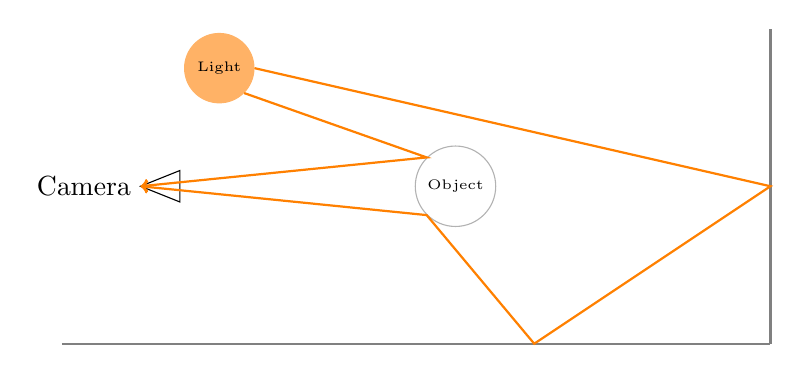
\begin{tikzpicture}
\draw[gray, thick] (-1,0) -- (8,0); %floor
\draw[gray, thick] (8,0) -- (8,4); % wall
\node[draw, circle, minimum size=1cm, draw=gray!60] at (4,2) (obj){\tiny Object};
\node[draw, circle, minimum size=5mm, draw=orange!60, fill=orange!60] at (1,3.5) (sun){\tiny Light};
\draw[black] (0,2) -- (0.5,2.2) -- (0.5,1.8) -- cycle node[anchor=east] {Camera}; % camera
\draw[->,orange,thick] (sun.south east) -- (obj.north west) -- (0,2); %direct ray
\draw[->,orange,thick] (sun.east) -- (8,2) -- (5,0) -- (obj.south west) -- (0,2); %indirect ray


\end{tikzpicture}
\label{raytracing}
\caption{The direct illumination is a combination of the light source properties and the object material. The indirect ray is a combination of the light source properties and the material of all the surfaces it collides with}
\end{figure}
\end{center}
\subsection{Light}
The material of a surface defines how it reflects or absorbs incoming light, and as a result characterizes its colour under different lighting conditions. In the physical world, no surface is perfectly even on a microscopic scale, making the angle and intensity of photon reflections at different wavelengths difficult to predict. Furthermore many photons are actually absorbed by the material depending on it's colour properties and the lights wavelength. Visible light is made up of a vast supply of photons, which can even be considered as a wave with properties like wavelength or amplitude. If we consider light on a macroscopic scale it is far easier to predict and represent. We often use the concept of 'colour' to refer to the wavelengths of light which an object reflects, where lighter objects reflect more wavelengths and darker objects reflect fewer, and absorb more photons. It is essential to note that the colour something takes on is actually representative of the wavelengths of light that it reflects towards the light sensing device, be it an eye or a camera. Very smooth objects such as mirrors reflect most wavelengths, at very predictable angles, and so take on different colours depending on the viewpoint, wheras some materials tend to reflect similar wavelengths in all directions. These behaviours are captured in the \textit{Rendering Equation}, formalized by Immel et al. \cite{Immel:1986:RMN:15886.15901},
\[L_0(x, w_0, lambda) = L_e(x, w_0, lambda) + \int_{ohm}{f_r(x, w_i, w_o,lambda)L_i(x, w_i, lambda)dw_i}\],
which Computer Graphics attempts to approximate to produce the correct pixel colors. We can see from this equation, that if we have understanding of the material of a surface, and the surface normal, we can derive some knowledge of the incoming light from the resulting colour.
\subsection{Materials}
In Computer Graphics, materials are often referred to as having \textit{Diffuse} and \textit{Specular} properties, which capture the aforementioned behaviour. This is in fact an approximation that allows for the efficient rendering of surfaces, though does not capture the light behaviour perfectly. Diffuse refers to the wavelength, or colour, of light that is reflected off a surface equally in every direction. This can be thought of as the 'base colour', that is somewhat invariant to the viewpoint of the observer. A material that is entirely diffuse is often reffered to as \textit{Lambertian}. Specularity refers to how reflective an object is, and is often used to approximate the light being reflected directly from a light source towards the observer. The \textit{Phong Shading} model combines these two elements to roughly represent a variety of materials, under the assumption that reflective materials have a dominant component that can be modelled as a mirror. For example an unlaquered wooden panel will be very unreflective and may contain no specular component at all, as its colour remains fairly consistent when observed from every direction. On the other hand a plastic ball will have a dominant colour but also reflect a lot of the incoming light, which is modelled as a combination of the incoming light direction and the surface angle. Modern Raytracing makes use of a far more accurate model called a \textit{Bidirectional Reflectance Distribution Function}, which defines a probability distribution function. This function gives the probablity of an incoming photon with angle of incidence i, reflecting with an angle of reflectance j. Over many photons this is able to accurately capture the reflective behaviour of a surface, and is often used in combination with properties like \textit{Albedo} and \textit{Subsurface Scattering} to result in an almost photorealistic surface. It is this complex reflection bahviour that makes estimating the light on a surface difficult, and why most solutions reduce the problem of lighting estimation to lambertian surfaces.
\subsection{Indirect Illumination}
A product of the reflective nature of surfaces results in \textit{indirect lighting}, an effect that is extremely difficult to capture in real-time rendering. The incoming light on a surface is made of photons arriving directly from light sources as well as photons being reflected from other surfaces, as demonstrated in \ref{raytracing}. Often when rendering is expensive it is appropriate to approximate the lighting in the scene to contain only \textit{direct} and \textit{environment} lighting. In this approximation, all objects are lit by the environment light, which represents an approximate light in all directions at all points in the scene. This is very cheap to render, as provided there is no direct lighting, all points on a surface recieve a constant amount of light. Direct lighting refers to lighting objects based on their proximimity to a given light source, ignoring shadows that would require calculating intersections between the light and the surface. Unfortunately this approximation results in very unconvincing images as in reality the light at a point is made up of all the photons being reflected from that point. The Phong shading model ignores the effect of photons being reflected many times within a scene, and so misses much of the subtle detail. A common way of calculating indirect lighting is \textit{Global Illumination}, which involves tracing the paths of many light rays from light sources as they are reflected within the scene. To save computation it is often performed in reverse, where rays are drawn from the camera and reflected a constant number of times. The illumination of the final reflection is then computed from the direct lighting, which is then passed between the reflected surfaces to achieve the approximate lighting at the original scene point. Global illumination is a very expensive procedure and innapropriate for real-time rendering, where other approximations can be used, such as \textit{Environment Maps} or \textit{Baked GI}.
\subsection{Digital Compositing}
%\begin{wrapfigure}{r}{0.25\textwidth}
%\includegraphics[width=4cm]{images/ar_example}
%"\caption{Example of Apple's ARKit lighting estimation in IKEA 'Place'.}
%\end{wrapfigure}
\textit{Digital Compositing} is an extension of computer graphics and computer vision, where virtual objects are rendered on a real video stream to appear as if they are part of the original scene. This creates additional challenges as many of the parameters that are used in computer graphics are not available. While the material and geometry of the added objects is known, the geometry and lighting of the real scene must be estimated or manually recorded beforehand. The latter option tends to be used in films, where the layout of the scene and camera movements are known to the digital artist. In this case the geometry of the scene can be measured and recreated in 3D modelling or CAD software for a virtual approximation.
\newline
Similarly, the lighting at points in the scene can be captured using a light probe, often a reflective sphere, and taking composite photographs at different exposures. This process results in an Environment Map which captures the color and intensity of all the incoming light at a single point. With this data, additional characters can be rendered entirely in the virtual space, interacting with the approximated geometry and being lit by blended combinations of light probes across the scene. Provided that the virtual camera moves exactly as the real camera, the added object can be masked and overlaid onto the original video of the scene.
\newline
While accurate lighting and geometry are enough to render a single accurate composite image, more is required for convincing video.  In computer graphics the appearance of a rendered object depends on the position and orientation of the camera. When using a real camera we need to know the position of the camera in the real environment.  In video footage, the camera tends to move, while the digital addition should remain in place in the 3D environment. To achieve this, the relative movement of the camera must be known, and compensated for. In the film industry, where the scene can be accessed beforehand, it is common to place high-contrast stationary markers within the scene. Once the footage has been collected, it is then possible to track the movement of these markers, and therefore the camera. If explicit markers are unavailable, it is possible to make use of features of the real environment as markers, such as high-contrast patterns on carpets or walls. This method is less robust, as often scenes may not contain enough stationary features to accurately track the camera. This is a significant difficulty in AR, with recent commercial solutions making use of the intertia sensors available in mobile devices.
\newpage
\section{Depth Estimation}
To estimate the lighting in a scene, it is important to have some understanding of the geometry within it, to exploit reflectance, shadows and environment context. Our work makes use of the parallax effect, taking inspiration from computer vision techniques for depth estimation from stereo imagery. Here we briefly cover how depth, and therefore geometry can be calculated.
\begin{figure}[H]
\centering
\includegraphics[width=8cm]{images/Stereo_Matching}
\caption{Example of Stereo Imagery. Points that appear further apart in the 2 camera places are further away from the camera due to parallax.}
\end{figure}
\subsection{Depth Cameras}
One of the most important components for scene understanding tasks is that of geometry. In the field of robotics especially, it is vital to be able to understand the placement of obstacles within the scene, while being tolerant of material and lighting changes. This problem is often paired with the task of motion or camera tracking, such that an actor can understand how they fit in 3d space. Furthermore, many of the techniques for lighting estimation previous mentioned require some understanding of the geometry of the scene. Geometry estimates tend to come in the form of depth and surface normals, which represent the distance from the camera and the surface normal direction (usually in camera space) for every pixel on the screen.
\newline
One method for collecting depth information is to use a depth camera, with specialized hardware to calculate depth for every pixel. An example of this would be the Microsoft Kinect camera, popular in computer vision tasks for its low cost. This calculates depth by projecting a pattern of infrared points onto the subject, and measuring how the distance between the points changes as objects move within the scene. For many cases this is inpractical, as the depth resolution is limited, and it's reliance on IR makes it unusable outside. It is however an excellent tool for collecting ground truth depth data for other systems \cite{Khoshelham_accuracyand}.
\newline
Another approach for capturing depth information is the use of stereo cameras, which record two seperate images of the scene. If the relationship between the two cameras is known, and the views of the cameras intersect, the epipolar constraint can be used to calculate the distance of every point from the camera. If the translation between the two cameras is known, this can be made easier by using \textit{rectified images}, such that the two views share a common plane. In this case, the center point of each camera view projects onto a unique point in the other's view. If corresponding image points can be found, the epipolar constraint can be used to find the exact projected 3D point. Even if the camera properties are unknown, if enough matching image points can be found, at least the relative depth of the images can be calculated.

\subsection{Stereo Matching}
Finding matching points between two images is a difficult problem, as some points may be duplicated or even occluded. This requires some form of stereo matching, often involving the comparison of image patches. One technique is to find the disparity of image patches, using a technique like \textit{Normalized Cross Correlation}, but this is very slow, and the accuracy of the results depends on the size of the image patch. Similar block-matching methods that compare pixel values like \textit{Sum of Squared Differences} or \textit{Sum of Absolute Differences} can be used but suffer the same accuracy penalty. There is a tradeoff in most stero matching algorithms between reliability and accuracy, as detecting the movement of single pixels is difficult, as on flat surfaces the value may not change for large regions. Furthermore, small image patches are easily affected by changes in lighting and material. On the other hand large sizes can only calculate a lower-resolution depth image. More modern techniques such as \cite{7780983} use CNNs to extract features at different granularities, before attempting to find the disparity between them. This has shown to be incredibly effective, combining the effects of global methods and block matching. It is this technique that we aim to exploit in our work to get a better understanding of scene depth, and therefore normals and reflectance.
\subsection{SLAM}
Stereo matching, or Disparity mapping is used to find the depth of points within a scene, from a single view pair. However it is often the case that we need an understanding of the geometry of an entire scene, which requires combining the calculated depth from multiple camera transforms. If the stereo cameras can be tracked, then it is possible to combine the calculated depth information to build a point cloud, or 3d point representation of the scene. This can be achieved with \textit{Simultaneous Localisation and Mapping}, which combines depth estimation with camera tracking. SLAM involves finding salient features between successive camera views to track the camera movement. When the movement between two frames is found, the markers can then be used as 3D points in a point cloud, along with the depth information calculated from the stereo cameras. It is also possible, if difficult, to perform monocular SLAM, using a single camera. As with camera tracking, this usually involves a combination of markerless tracking and intertia sensors. SLAM on mobile devices with standard cameras is still a mostly unsolved problem, as estimated markers tend to be sparse and point clouds computationaly expensive.
\section{Machine Learning}
The lighting in a scene is determined by complex relationships between geometry and materials. Hand crafting a robust system that is able to take into account different image features like shadows and reflectance, without relying on limiting assumptions is difficult We approach this problem using Deep Learning, where we train a model to learn the optimal features to capture the input and reproduce a lighting output.
\newline
\subsection{Deep Learning}
If we wish to predict a more complicated lighting model we must be able to take into account many more features than what we can feasibly define by hand. In this case we can look to the field of AI, and explicitly \textit{Convolutional Neural Networks}. In the field of AI it is possible to train a model without explicit features, by using an approximation of neural dynamics in real brains. In broad terms, we programmatically create a series of connected neurons in a layered structure, with each neuron having a number of inputs and some number of outputs. The neurons have a very simple behaviour - they multiply each input by some 'weight' and provide the accumulated result as the output:
\[y_k = \sum_{j=0}^{m}{w_{kj}x_j}\]
By training on known results we can adjust these weights so that the final neuron layer (which matches our desired output data shape) contains the desired output.
\newline
Convolutional Neural Networks are a recent development in AI that allows for reasonably fast AI models that take images as input. Rather than having a neuron for each colour of each pixel, we can instead learn the weightings for a \textit{convolution}. A convolution, in this context, is a function which can be passed across an image to extract features,
\[\sum_{n_1=-s}^{s}{\sum_{n_2=-s}^{s}{f[n_1, n_2]\cdot g[x-n_1,y-n_2]}} \]
and often resembles a SxS matrix. Convolutions are used frequently in computer vision, as they are an efficient way of computing many popular image features such as \textit{Harris Corners} or \textit{Sobel Edges}. In a CNN we intend to learn the weights of many convolutional matrices to quickly extract featured from the input image. Furthermore we are able to pass further convolutions across the results from previous convolutional layers to learn more complex features. For example the first layer could extract edges while a second layer extracts the presence of 'X' shapes. CNNs make it possible to train deep and complex models on image data, resulting in robust models that often vastly outperform their traditional ML counterparts.
\newline
The performance of CNNs is heavily impacted by the choice of metrics used to decide the weights and behaviour for each neuron. When given inputs and weights a neuron may or not fire depending on an \textit{activation function}. In biological neurons, this is a complex nonlinearity that is difficult to efficiently capture in artificial neural networks. Instead we use approximations like 'Relu',
\[f(x) = max(0,x)\]
to decide whether to fire after calculating the output value. Furthermore during training it is important to consider how to adjust the weights to converge on the optimum. For this we use a \textit{Loss Function}, which computes an error value given the desired, or ground truth, value and our models prediction. The rate of change of this error is then used to iteratively adjust the weights of each neron based on its influence.
\subsection{Image Regression in Deep Learning}
The prime application of CNNs has been in image classification, where the model must distinguish between a set number of classes. However it is possible to use CNNs for regression tasks that output other images using the concept of \textit{deconvolutional} layers. These learn an interpolation matrix that increases the dimensionality of the input. Popular image regression architectures often involve a series of convolutional layers followed by a series of deconvolutional layers. The aim of the convolutional layers is to learn a deep representation of the content of the image, often removing the original spatial dimension. Rather than 'shallow' features like edges or colours, these features ideally represent some understanding of the scene such as presence of some object or shape of the environment. The deconvolutional layers can then interpolate this data into a new image that will often share many common features with the original. For example in style transfer, the convolutional layers attempt to extract the content of the image while the deconvolutional layers interpolate the image features with weights representing some artistic style. In our work we use a CNN to extract learned image features from input images of the target object, before making use of deconvolutions to extract a lighting representation. The purpose of the intermediate layers is to learn to approximate the lighting without explicit constraints.

\subsection{Training Data}
The difficulty in the application of CNNs often lies in the \textit{training} stage; while a deep enough network should be able to learn a mapping for any function, the difficulty in providing data to capture every case increases with the problem complexity. If a network is trained to recognize images of dogs, it will only be able to learn features from dogs that it has seen as input. As a result, if a new dog is provided that lacks some of the features of the training data, it may be missclassified. Regression tasks in particular attempt to learn a complex funtion and so need a vast amount of training data to be able to generalise. This becomes problematic where the training data is hard to collect and classify.
\begin{wrapfigure}{r}{0.3\textwidth}
\includegraphics[width=5cm]{images/example_synthetic}
\centering
\caption{An example of syntethic data used for our work.}
\label{fig:synth}
\end{wrapfigure}
In the case of image classification, many photographs can be taken and marked with their intended class. With image regression this can become an extremely laborious task as the desired output needs to be extracted by hand. Often there are large datasets already available that can help speed up the process, especially if the datasets are labelled, or if features can be extracted by hand. However it is simply necessary to manually create a dataset to train a network to face a new task. Fortunately there are still some steps that can be taken to accelerate this process, such as data augmentation. This usually involves manipulating some training inputs in such a way as to introduce variances while maintaining the classification, and can greatly increase the amount of data available.
Another approach is to create synthetic virtual data, by rendering new images, such as the one in \ref{fig:synth}. It is important to note however that the synthetic data must be accurate enough such that a model trained on it can generalise to real world data. It is often sensible to mix real world and synthetic data when training a model for the best results. Lighting information is very arduous to capture manually, and so we use synthetic data for our learning task.

% -----------------------------------------------------------------------------

\chapter{Technical Background}
\label{chap:technical}
\section{Commercial Lighting Solutions}
\begin{figure}[H] 
\centering 
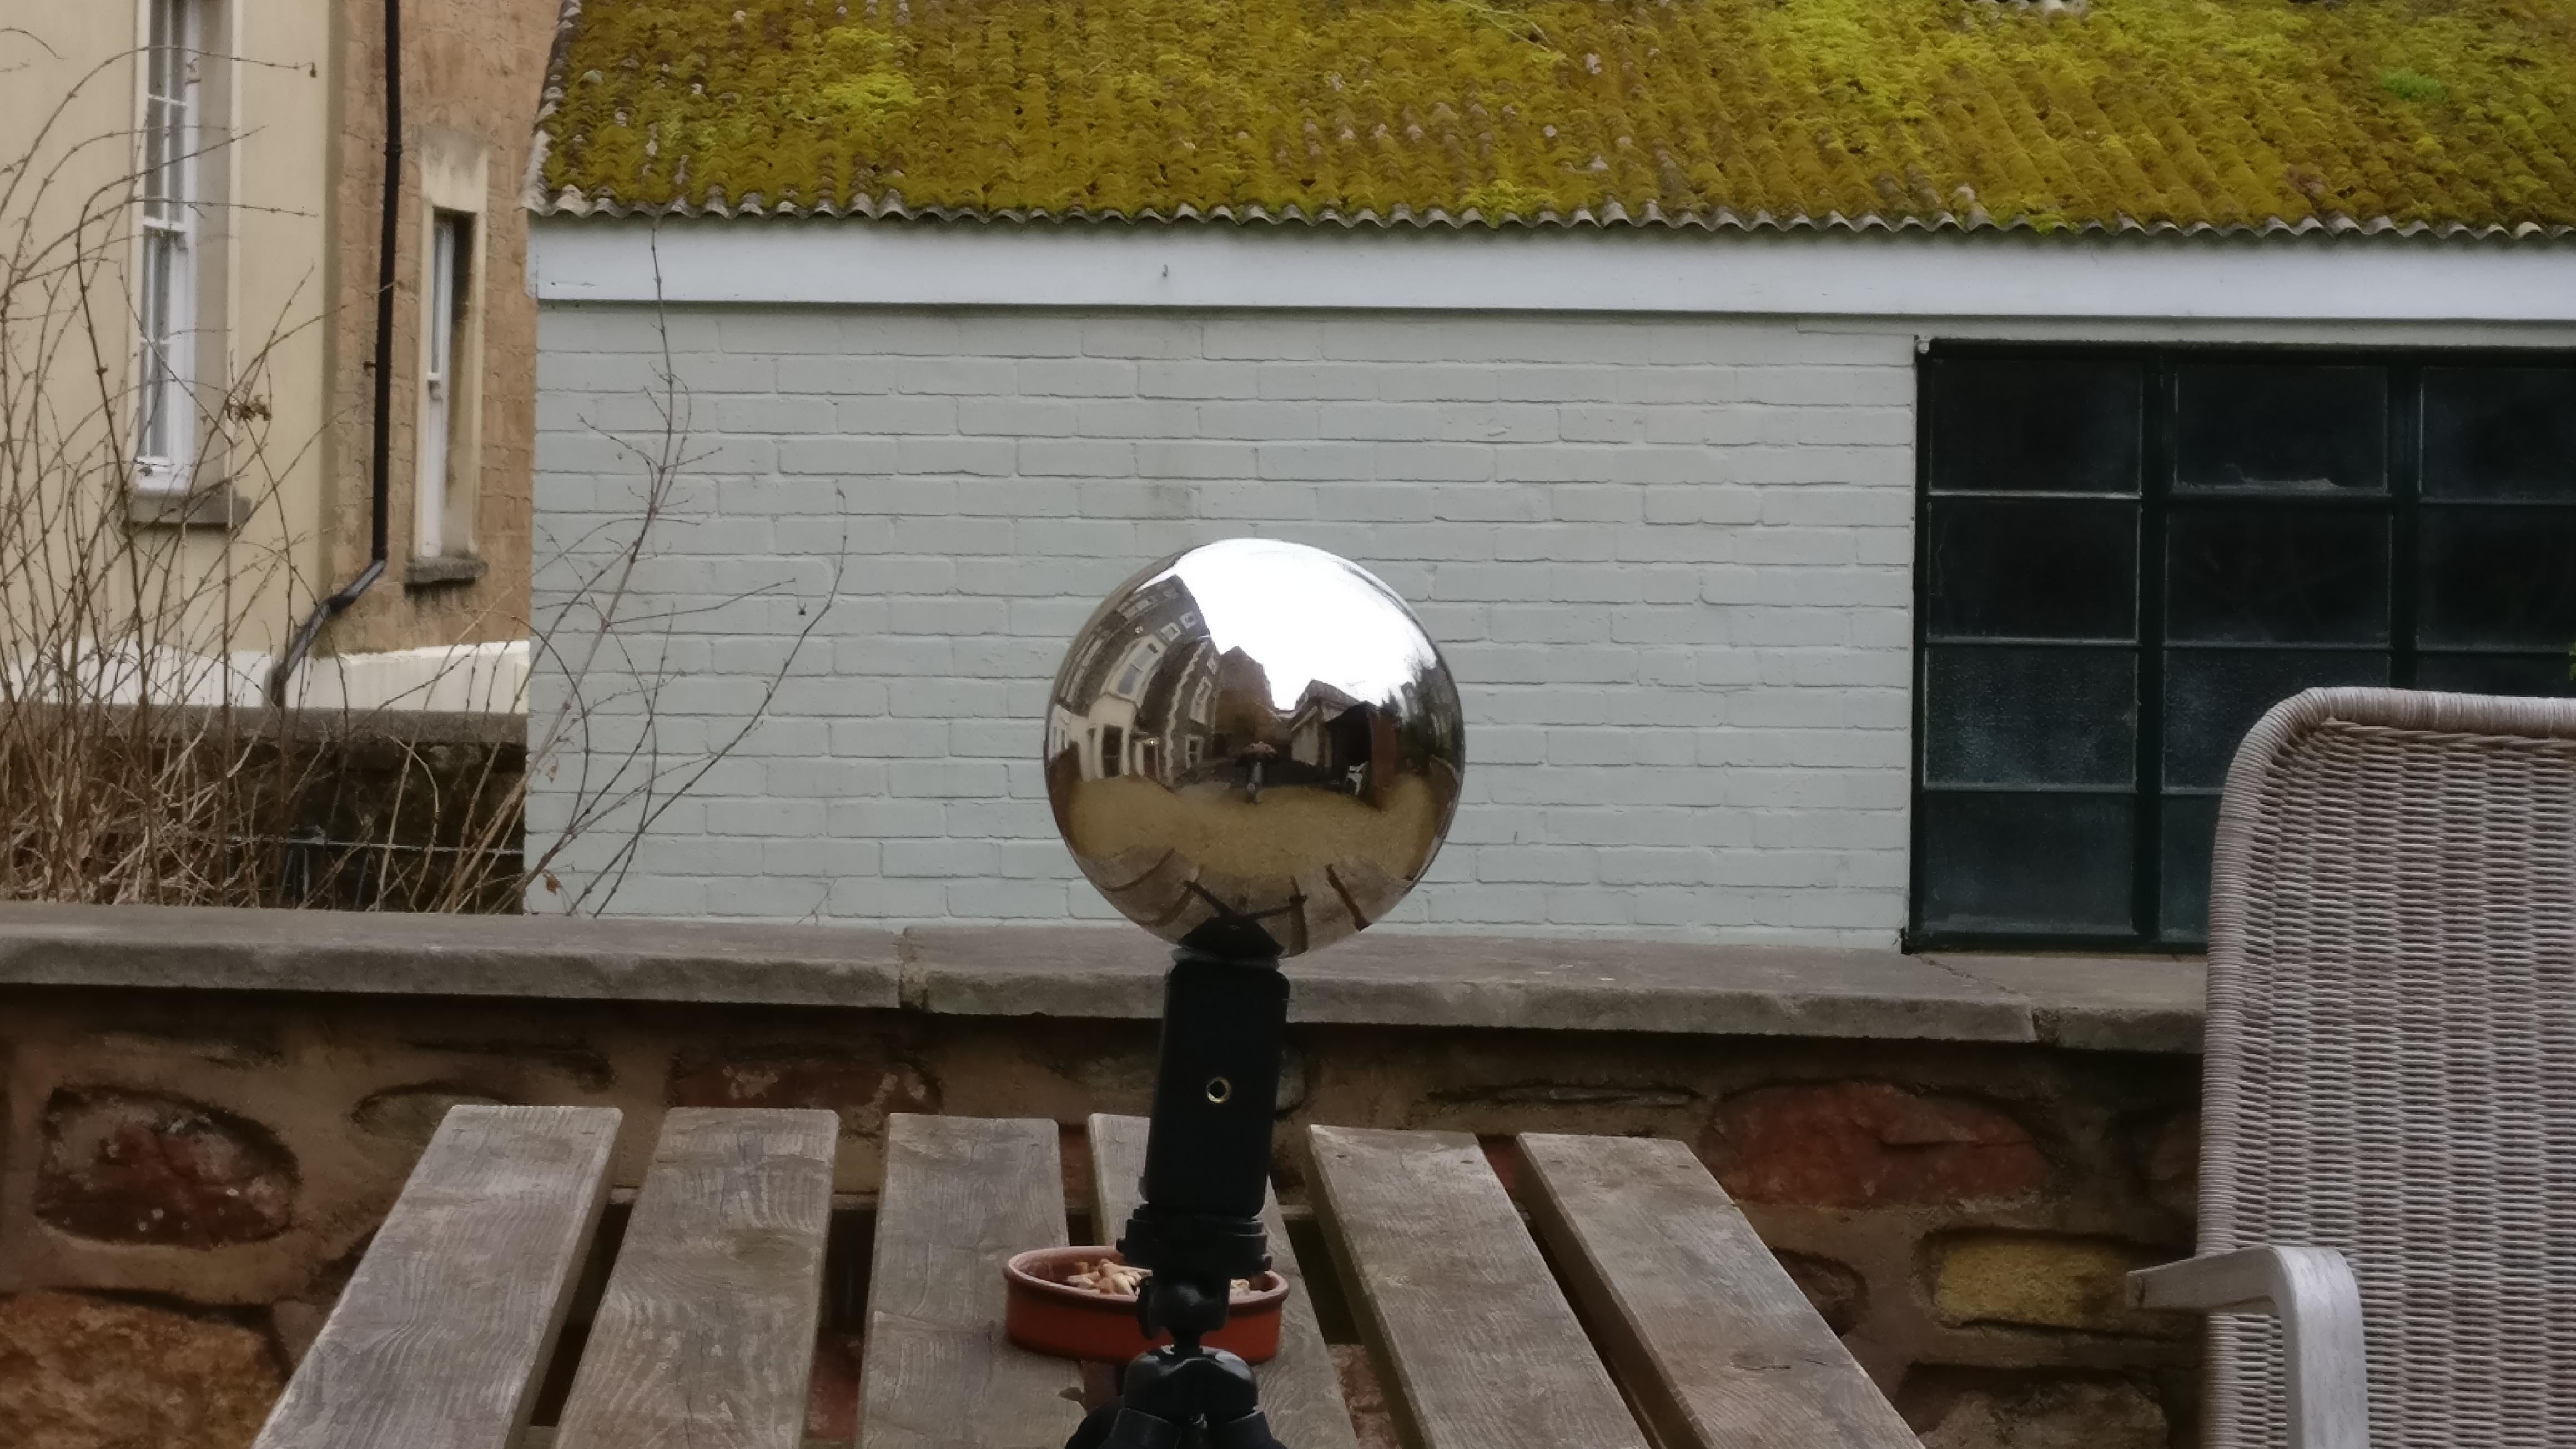
\includegraphics[width=7cm]{images/envmap} 
\caption{A mirror sphere used to capture Environment Maps} 
\end{figure} 
\subsection{Light Capture}
Lighting solutions in the motion picture industry tend to involve precalculating or precapturing the lighting in a scene before adding virtual characters. In the film 'Flight of the Navigator', Randal Kleiser first demonstrated the technique of reflectance/environment mapping in a feature film \cite{navigator}. Here the reflectance was computed using a simple rectangular photograph, although more accurate implementations used spherical photographs of a gazing ball. Later films used a semi-automated system for capturing HDR environment maps using a rotating fisheye-lens camera. Once placed, the camera was able to take shots at multiple angles and at a range of exposures, before compositing the shots together to produce a usable HDR lighting map. Often these HDR maps are not used in isolation, but along with footage of a proxy for the virtual addition, so the filmmakers can qualitatively measure how the materials react with the set lighting. These techniques allow filmmakers to capture an approximation of lighting with limited camera equipment and makes it easier to create complex panning and dolly shots of scenes with real and virtual elements, which would otherwise require a green-screen. Over time, camera equipment has become more advanced and it is faster to take high quality shots at multiple exposures. As a result, later films such as 'The Curious Case of Benjamin Button' are able to utilise multiple lighting probes to illuminate characters. By taking lighting samples across the scene, virtual characters can then be lit partly according to their position in the world by blending environment maps together. This creates a more convincing final render as the approximate indirect lighting from nearby objects becomes more apparent. The downside of these hollywood techniques is that the lighting data must be captured beforehand for every environment used. This is a long, laborious and expensive process as the cameras required to take accurate shots at different exposures need to be extremely accurate to produce correct composites. It is also important to note that compositing images is difficult and also requires human input to match black levels, tones and camera properties that are hard to automate.
\begin{center}
\begin{figure}[H]
\centering
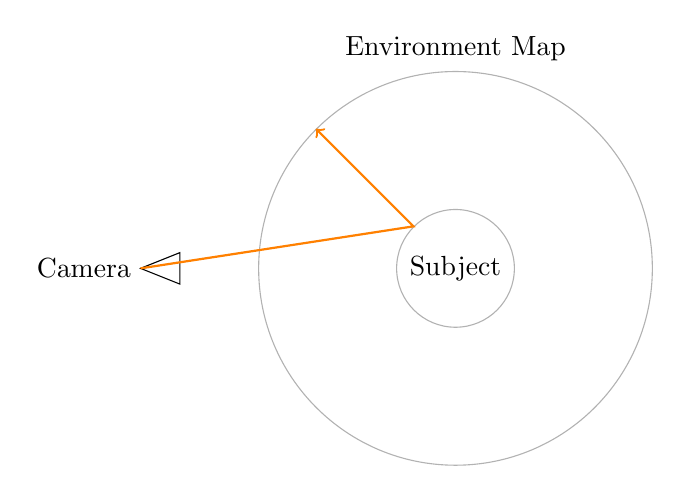
\begin{tikzpicture}
\node[draw, circle, minimum size=5cm, draw=gray!60] at (4,2) (env){};
\node[above] at (env.north) {Environment Map};
\node[draw, circle, minimum size=1cm, draw=gray!60] at (4,2) (obj){Subject};

\draw[black] (0,2) -- (0.5,2.2) -- (0.5,1.8) -- cycle node[anchor=east] {Camera}; % camera
\draw[->,orange,thick] (0,2) -- (obj.north west) -- (env.north west); %direct ray


\end{tikzpicture}
\label{environment map}
\caption{An environment map being used to render a sphere to the camera. This process is reversed with a perfectly reflective sphere to obtain the environment map}
\end{figure}
\end{center}

\subsection{Light Estimation}
Recent commercial AR platforms do contain some level of lighting estimation from input video data. Apple's ARKit is able to estimate the colour and intensity of the ambient lighting in some scenes \cite{arkit1}, by analyzing the pixels of the incoming video frame. This technique adds some realism to AR applications, as objects can be dimmed or brightened with the scene, so as not to stand out. However this is a very rough estimate of lighting, and contains no directional information or approximation of indirect illumination  Google's ARCore has similar functionality, taking an average of the luminance values across the video to estimate the intensity \cite{Debevec:1998:RSO:280814.280864}. It is possible to estimate the light direction from a face tracking scene however, by using the tracked face as a light probe. By using a face, the application is able to restrict the possible lighting scenearios to a range of likely geometries and materials that make up human faces. The platform is able to produce not only the primary light direction and intensity, but also an approximation of the environment lighting as spherical harmonics. While incredibly useful for some application such as the retouching of portrail photographs, the technique is not robust to different scenes as it relies on the approximation of some known geometry.
\begin{wrapfigure}{r}{0.4\textwidth}
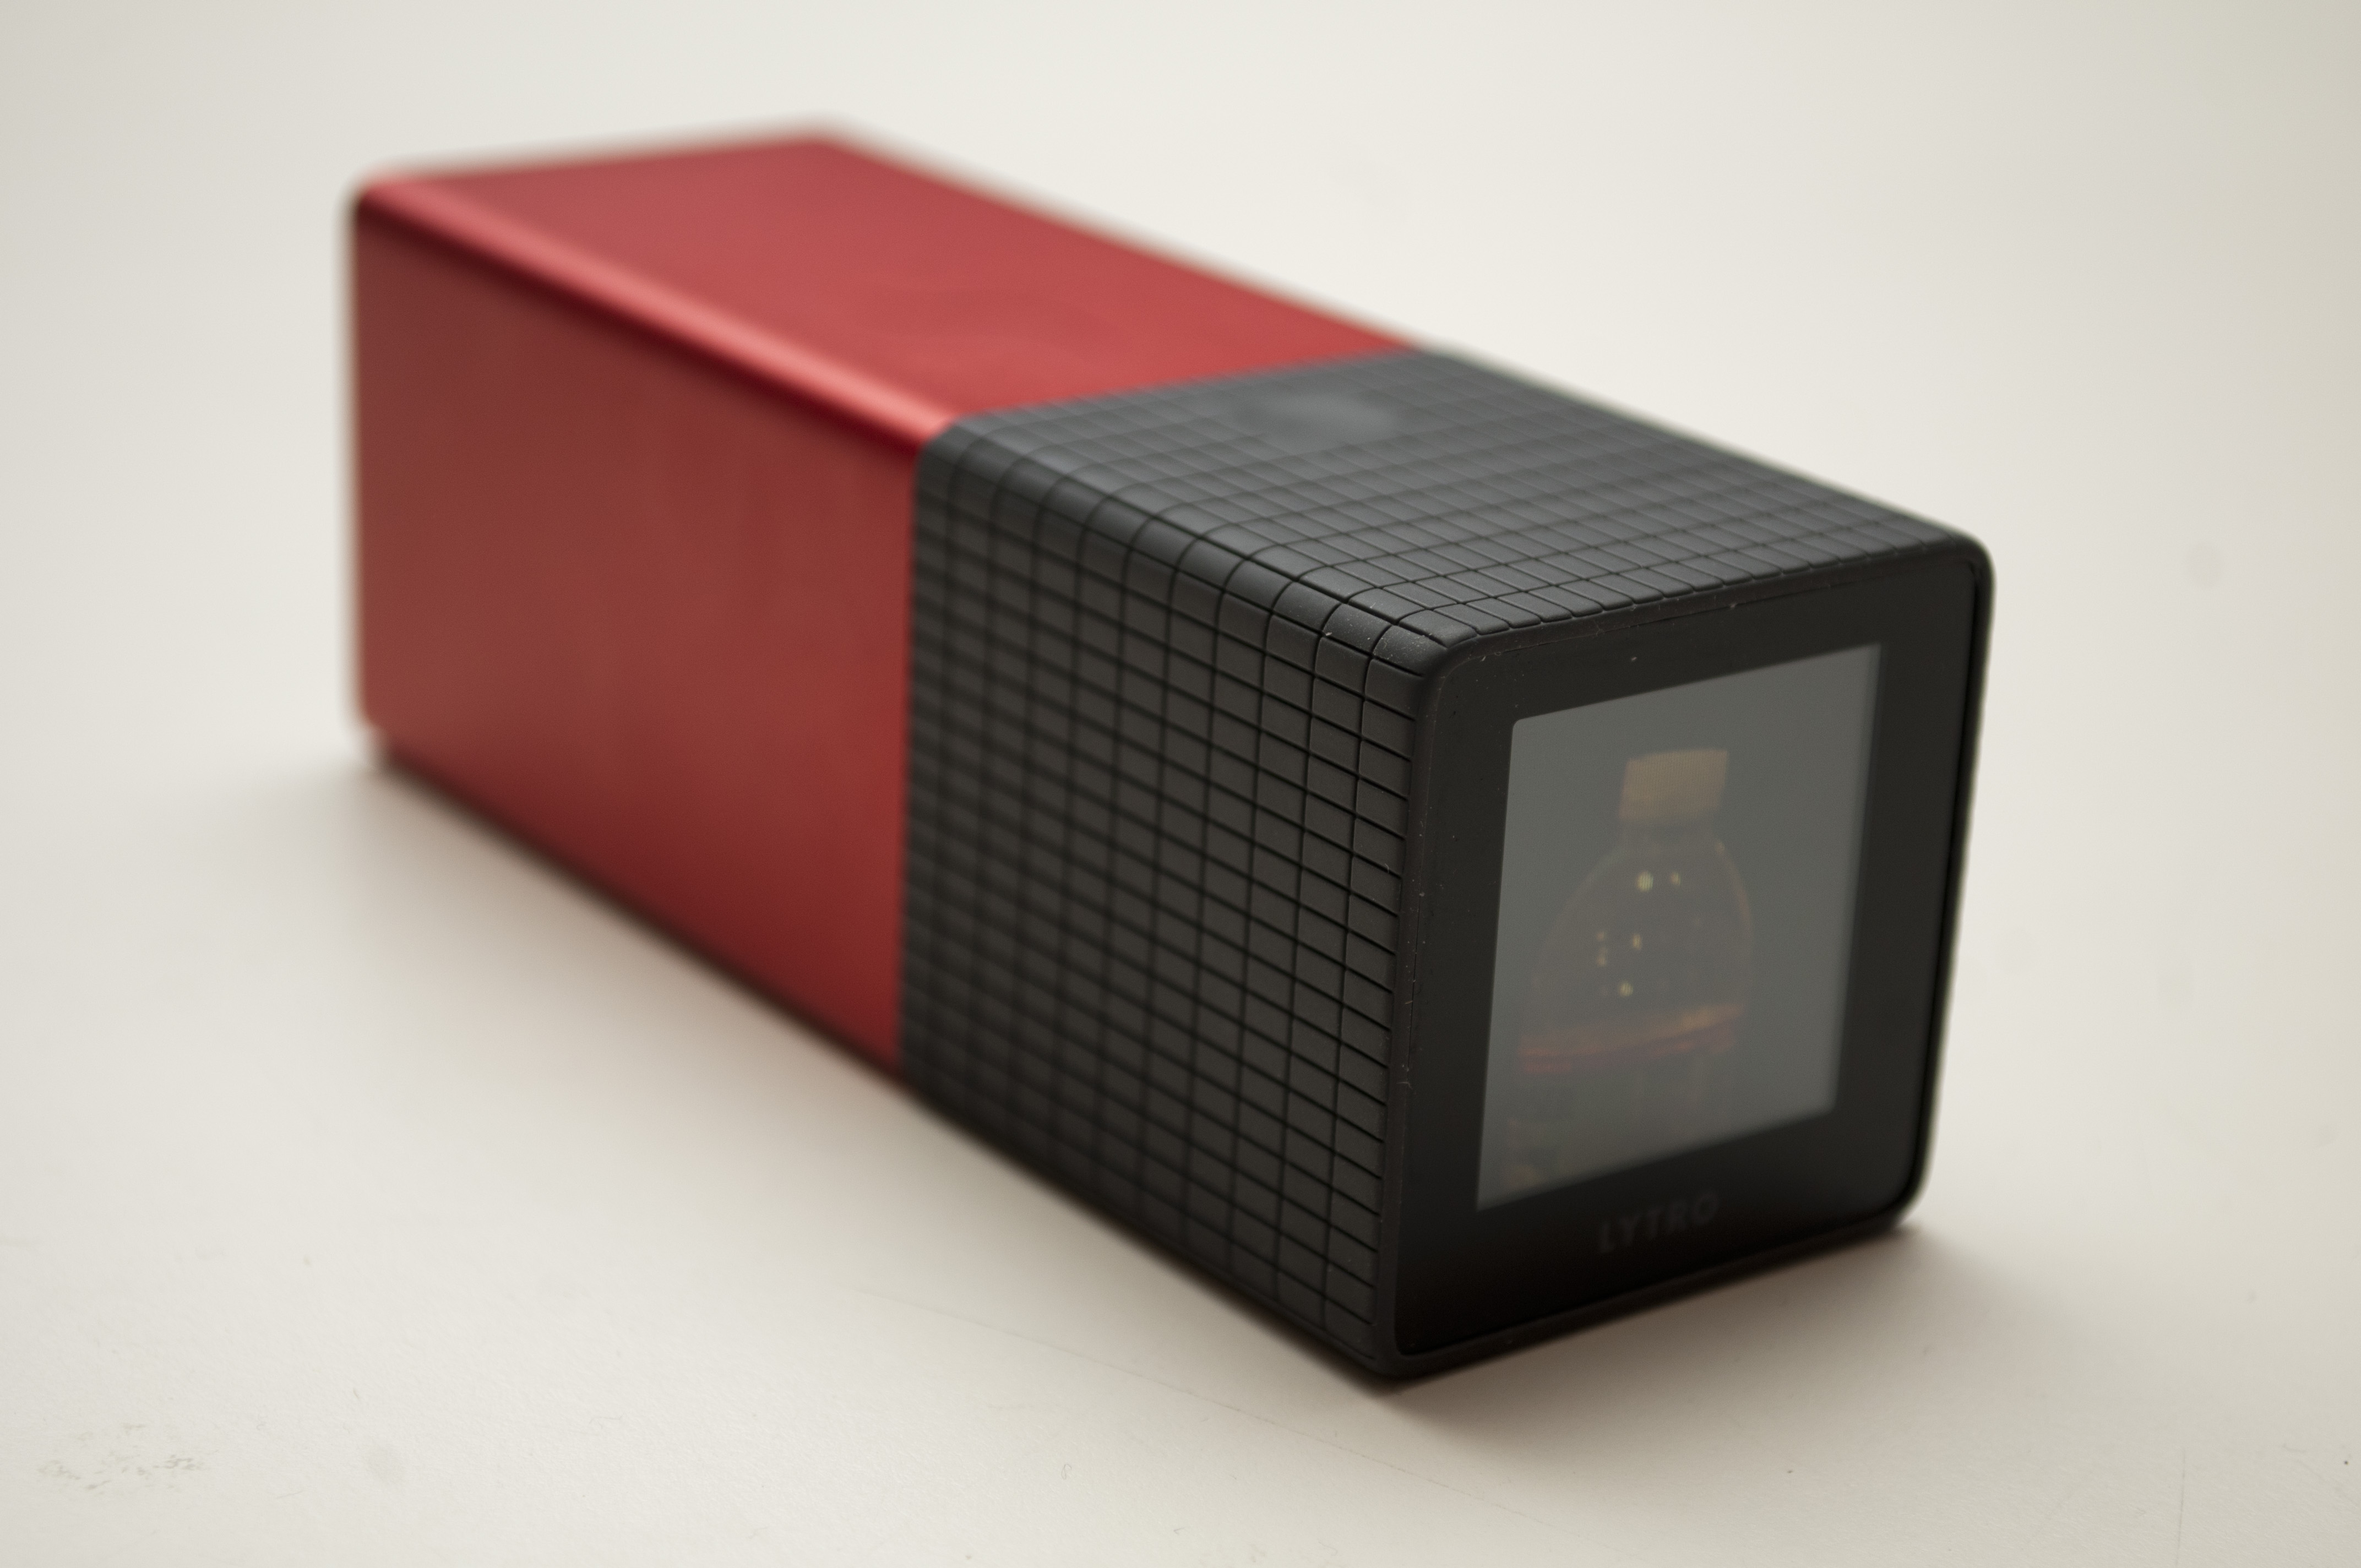
\includegraphics[width=5cm]{images/lytro}
\centering
\caption{A commercial light-field camera from \textit{Lytro}}
\end{wrapfigure}
\newline
Upcoming AR applications are experimenting with new methods of integrating the scene lighting with virtual augmentations. Magic Leap is making use of tailored hardware called a 'Light Field' camera, which involves the use of an array of microlenses to capture additional information from the scene. Each microlens is able to capture information from multiple camera points, so that extra depth and lighting information can be extracted from the frame. This is a significant improvement on IR depth cameras such as the Microsoft Kinect, which can't be used outside. By extracting depth, and therefore surface geometry information, it is far easier to reason about the reflectance of objects within the scene and estimate the lighting. However, light-field cameras are extremely expensive and inpractical for mobile AR. Most mobile devices contain normal high quality cameras as well as accurate intertia sensors, which can be used in combination with stereo matching for a similar depth estimation model.
\section{Lighting Estimation Research}
\subsection{Direct Lighting}
Early techniques for lighting estimation were able to find the direction of a single primary light source, under significant constraints. In \cite{990650}, Peter Nillius and Jan-Olof Eklundh were able to estimate a single light direction, provided the input image contained an appropriate lambertian surface.
\begin{wrapfigure}{l}{0.5\textwidth}
\includegraphics[width=5cm]{images/Contour}
\centering
\caption{A self occluding contour. The surface normal is orthogonal to the camera ray, and so the brightness of resulting pixel compared to the rest of the surface gives a good indication as to the illumination arriving from that direction.}
\end{wrapfigure}
By making use of an 'occluding contour' it is possible to infer some detail of the geometry, as the surface of the visible edge of a contour that occludes itself will always be perpendicular to the view direction of the observer. Using the lambertian lighting model, along with the edge intensity it is possible to make a prediction using a bayesian network for the incoming light direction. This is a simple method that exploits inherent properties of real geometry, but has too many prerequisites to be practical. While it captures direction, it also ignores colour, intensity and any indirect lighting. Similarly, Varma demonstrates a technique to estimate the lighting direction from textured images \cite{1315030}. If the surface is constrained to be a gaussian surface with uniform albedo, the incident light direction can be estimated by the shadows cast by the height changes in the material. While also very constrained, it is shown that even strict models can generalise to produce useful results in this field.
\newline
There has been some work in inverse lighting specifically for the rendering of AR objects, notably that of \cite{Aittala2010}. In this work the user must simply provide a ping-pong ball, representative of a lambertian sphere, while the least-squares algorithm is performed on the lighting equation, using features of the sphere as constraints. This results in an approximation of illumination as a series of point lights and spherical harmonoics which can practically be used for rendering. The downside however is that the process of presenting the system with a known ball can take upwards of 20 seconds, and the resultant lighting is suitable for only primarily diffuse objects. This does however demonstrate how powerful even basic knownledge of the geometry and material of the scene can be for deriving the lighting.
\subsection{Outdoor Lighting}
In \cite{Lalonde-2009-10350}, Lalonde et al. are able to estimate a more complete set of parameters for environmental lighting from single outdoor photographs. By segmenting the image into sky, ground and vertical surfaces, and extracting features like shadows, the authors are able to reliable predict the sun's position. While very robust for outdoor applications, this approach does not consider light intensity or colour. Furthermore, the reliance on outdoor scenes restricts its usage in AR.
Scott Wehrwein et al. demonstrate a technique for sun direction and shadow detection from multiple input images \cite{7335515}. They use illumination rations to extract shadows, after constructing a sparse 3D representation of the scene from stereo matching of multiple images. By exploiting shadow boundaries on the derived surface normals, it is then possible to determine the light direction. This work shows how multiple views can be used to infer knowledge of the geometry of the scene, to make the problem of lighting estimation more constrained. However, like previous work it assumes a perfectly lambertian surface and clear outside conditions, restricting the possible lighting conditions significantly.
\subsection{Shadows}
It is clear that estimating a full representation of the illumination within a scene is very difficult given the number of unknowns. However predicting only the direct light sources is still very valuable, as this makes up the majority of the light within a scene, and can be combined with image colour values to give an approximation of the indirect lighting. Shadows are a good indicator of the direction and intensity of direct lighting. They not only give some indication of direction based on shape, but also the intensity through the contrast of colour values between areas that are shaded and unshaded. Takahiro et al. demonstrate techniques for recovering illumination from shadows in \cite{1315013}. This work compares two methods, \textit{Spherical Harmonics} and \textit{Haar Wavelets} for estimating the illumination from cast shadows on known geometry. Spherical Harmonics are function defined over a whole sphere, and are useful for defining the light reflectance at a point, as in Global Illumination. The work demonstrates how this method fails to capture higher frequency illumination values, and presents \textit{Haar Wavelets} as an alternative. This method is able to approximate functions as a series of linear combinations of Haar functions, and is able to more efficiently capture a higher range of light frequencies at a point.
\subsection{Experimental Methods}
An interesting approach from Microsoft Research \cite{xia} attempts to reconstruct the shape and reflectance of an object from a video with known motion and camera pose. This is achieved by decoupling the estimation of geometry from the estimation of illumination, and refining initial estimates over a series of video frames. While the lighting is not known in the scene, the camera pose and motion must be known and so this work is only applicable under carefully controlled environents. However it effectively demonstrates how multiple views of an object can be used to refine predictions of scene understanding, under the reasonable assumptions of static lighting, material and per-object geometry.
\newline
An emerging trend in lighting estimation research is the use of 'light fields' as a way of representing the light on an entire scene. A light field represents the radiance of light flowing in each direction in each point in space, resulting in a 5D function. Capturing and storing light field data is difficult as for a given area, light must be sampled in all directions at all points, which is impractical using traditional cameras. The use of microlens light-field cameras, which sample incoming light rays at a range of angles, has made capturing light-fields much less costly, resulting in datasets becoming available such as that of \cite{hazirbas17ddff}. Light fields require immense quantities of storage capacity and contain far more light information than is required in the field of AR, making their use inpractical. Instead most work has been centered around the estimation of light at a single point, either at the camera view or in the scene, that can be seen as a sparse sampling from the light-field.
\begin{figure}[H]
\includegraphics[width=3cm]{images/antinous_rgb}
\includegraphics[width=3cm]{images/antinous_lf}
\centering
\caption{An example of the extra data captured by light-field imaging.}
\end{figure}
\section{Deep Learning for scene understanding}
\subsection{Geometry Estimation}
To calculate the lighting of a scene, some assumptions or approximations must be made about the material or geometry to constrain the problem. It is therefore important to consider previous techniques to extract these features from images, especially geometry estimation which has significant applications in the field of robotics. In 2015, David Eigen et al. demonstrated a CNN approach to estimate depth, surface normals and semantic labels from single input images \cite{7410661}. Here they use a 'multi-scale' architecture, where outputs from early features passed as input to later deconvolutional layers, as well as subsequent convolutional layers. Multi-scale features can often lead to faster inference as important features are 'short-circuited' closer to the output, reducing the need for large deep layers at inference time \todo{Citation needed ;) }. The results of this work are extremely promising, and suggest that a single RGB image may be enough to infer a complex understanding of the scene. If it is possible to understand variations in the illumination and material in a scene to find geometry then it follows that it is possible to understand geometry and material to find illumination.  However the network shown is very deep and trained primarily on indoor scenes. Its use in the field of AR is limited, as the hardware is much more limited in terms of GPU resources. Furthermore while the network is able to predict depth and surface normals on a large scale, successfully finding walls and floors, it struggles with more complex geometry. Some progress has recently been made to improve performance in geometry estimation by incorporating more traditional SLAM techniques. In their work, Luo et al. show increased performance in stereo matching by including a dot product step \cite{7780983}. In stereo matching tasks, two images are used to compute a disparity map, which corresponds to a relative measure of depth due to the parallax effect. This work uses a siamese network, where the same features are extracted from each of the two images. As a result, using a dot product computes a similarity between the two sets of feature outputs. This is equivalent to the \textit{Cosine Similarity} of the image vectors, provided they are normalized. This greatly reduces the number of layers that would otherwise be required to map the input image to output disparity map, while still producing accurate results.
\subsection{Synthetic Datasets}
With it's usefullness in robotics, geometry estimation has been a primary focus of scene understanding tasks. Geometry datasets are easier to source, with depth cameras becoming cheap and easily available. Other important information like material, texture, semantic class, albedo an many others are almost impossible to capture efficiently from real scenes using hardware. Instead these parameters must be hand labelled, which is expensive, slow and leads to noisy results. The recent availability of high quality synthetic datasets such as SUN-RGBD \cite{song2015sun} and the very recent Scenenet-RGBD \cite{McCormac:etal:arXiv2016} however, have provided more opportunities for learning scene parameters that are more difficult to retrieve from real scenes. For example, Rajpura et al. demonstrate how semantic segmentation networks can be improved by augmenting real data with the readily available synthetic data \cite{DBLP:journals/corr/abs-1709-00849}. Some networks must be trained entirely on synthetic data, such as that of Narihira et al. which utilises the syntetic MPI Sintel dataset to predict shading and albedo, which can't be captured by hand. Unfortunately, many synthetic datasets do not generalise well to real data, and it remains to be seen whether virtual scenes with the level of detail needed for lighting estimation can be rendered fast enough to be practical for research, although recent datasets appear promising.
\begin{figure}[H]
\centering
\includegraphics[width=16cm]{images/scenenet}
\caption{Example synthetic Scenenet RGB-D data, containing RGB, depth, semantic instance, semantic class and optical flow.}
\end{figure}
\subsection{Deep Learning for Illumination Estimation}
Most of the previous work has had to rely on significant assumptions for the scene to constrain the lighting to fit known phenomena, that can be exploited to estimate the illumination. It is clear that due to the unconstrained nature of the problem, that some assumptions about geometry, material and lighting must be made. Rather than making the required assumptions to fit a model, another approach is building a model to find and exploit assumptions from real data using machine learning. Given enough scene features and data it is possible to learn approximations and assumptions to produce a more robust model. In \cite{holdgeoffroy-cvpr-17}, Yannick Hold-Geoffroy et al. use a CNN-based technique to estimate sky parameters from outdoor photographs to a high enough degree of accuracy that virtual objects can be re-rendered. In this work, the output illumination model is constrained to the Hosek-Wilkie model with parameters representing the sun position, ground albedo and light wavelength. A dataset is then constructed by selecting small LDR sections of real HDR scene panoramas, resulting in a large number of sample photographs, and HDR lighting ground-truths. This work demonstrates extraordinary performance, but is limited in output format by the lighting model which is constrained to outdoor images with clear skies. This ignores the indirect lighting from scene objects and indoor scenes, but demonstrates how CNNs with the right data can be used to exploit more subtle image features to predict lighting.
\newline
There have been advancements in the field towards estimating the lighting in indoor scenes, such as that by \cite{Gardner:2017:LPI:3130800.3130891}. In this work, Gardner et al. use a very large dataset of indoor HDRI environment maps to train a CNN to predict the environment map at the cameras position. This environment map can then be warped to provide an approximate environment map for a given position. The resulting network is very accurate for predicting light direction and intensity, but fails to predict colours which must be provided for a user. Furthermore the network is very deep, making it difficult to deploy on mobile devices. While the warping operator user is innovative, it fails to accurately capture the lighting at points in 3d space, and instead provides a rough approximation. Finally, the produced lighting requires a manual tuning step if it is to match the scene in hue, though this is the still very promising work in the field of lighting prediction.
\section{Predicting Light Probes}
CNNs can exploit different features in a scene to determine lighting such as shadows or object reflectance. One example that uses the latter is 'Deep Reflectance Maps' \cite{RematasCVPR2016} by Konstantinos Rematas et al. In this work it is demonstrated that better accuracy can be achieved by constraining the CNN input to a specific feature, in this case a sparse reflectance map, provided the geometry is known. A reflectance map is mapping from surface normal direction to light reflectance in that direction. By taking the brightest pixel for every surface normal on an object, a sparse representation of it's reflectance can be built and fed to a CNN for interpolation. This work makes use of a large synthetic dataset but still results in good performance on real world data, allowing the researchers to then modify the shape of specular virtual objects while still maintaing a realistic surface appearance. An important feature of this work is that the researchers present results from reflectance maps produced from perfect surface normals, and from those produced by noisy estimated normals. It is demonstrated that the estimated normals are unsuitable for accurate reflectance mapping, and actually result in poorer predictions than a direct appearance-to-lighting network.
\begin{figure}[H]
\includegraphics[width=8cm]{images/reflectance}
\centering
\caption{The \textit{Deep Reflectance Maps} pipeline. Estimating the full reflectance map from the geometry and depth data allows for modification of the material.}
\end{figure}
This work was then extended for illumination estimation in 'What is Around the Camera', by using a precalculated sparse reflectance map in combination with a segmented background image. In this work, a full HDR environment map is predicted to a degree of accuracy that allows the superimposition of rendered geometry with fairly accurate lighting. Both of these works use a Convolutional-Deconvolutional approach to produce a new image as output. The limitations of this work however are due to required prior calculations rather than restrictive assumptions about the scene. While the network can handle objects of multiple materials, they must be segmented and seperate sparse RMs calculated. Furthermore the calculation of the sparse RM relies upon knowledge of the surface normals of the object being used. The researchers point to previous work \todo{Talk about this} on the usage of CNNs for surface normal and depth estimation but fail to demonstrate the accuracy of their work with these more noisy estimated surface normals. It is also apparent that there is significant data loss in the calculation of the sparse reflectance map, which makes significant assumptions about the object in question, ignoring the effects of shadows and how lighting changes based on both position and surface orientation.
\newline
These works demonstrate that if surface geometry is known, a network can be trained to accurately reproduce lighting conditions, using an object as a probe. However they point to 2 significant shortcomings that we attempt to address in this work. Firstly the use of sparse reflectance maps in isolation ignores a significant amount of useful information on the object that could be used to estimate the lighting. As a result, a direct approach of predicting illumination from a single image view can often outperform cases where the reflectance map is too sparse or the material is very diffuse. Secondly, modern surface normal estimation techniques from single images are not accurate enough to constrain the problem of lighting estimation. We believe that the use of a network that exploits multiple views of an object, provided the scene parameters remain constant, will be able to more accurately predict the geometry through learned stereo matching. Furthermore, a network that simultaneously learns geometry and lighting will be able to exploit more scene features such as shadows, that would otherwise be unavailable in an explicit reflectance mapping.
\newline
\footcite{https://www.disneyresearch.com/publication/face2light/}
\begin{figure}
\def\checkmark{\tikz\fill[scale=0.4](0,.35) -- (.25,0) -- (1,.7) -- (.25,.15) -- cycle;} 
\begin{tabular}{|c|c|c|c|c|}
\hline
Model & Geometry Prerequisite & Material Prerequisite & Direct Lighting & Indirect Lighting \\
\hline
Mirror Ball & sphere & mirrored & \checkmark & \checkmark \\
Nillius et al. & occluding contour & Lambertian & \checkmark & X \\
Varma et al. & Isotropic Gaussian Surface & Constant Albedo & \checkmark & X \\
Lalonde et al. & Outside with floor\& sky & X & \checkmark & X \\
Wehrwein et al. & Outside \& clear & Lambertian & X & X \\
\hline
\end{tabular}
\caption{Summary of current methods}
\end{figure}

% -----------------------------------------------------------------------------

\chapter{Implementing Prior Art}
\label{chap:execution}

\section{Deep Reflectance Maps}
It was important to reproduce the preceeding work, to assess its aplicability in the field of AR and create a fair benchmark for evaluating our new models and approach. We began with a reimplementation of \textit{Deep Reflectance Maps}, a recent work that demonstrated promising results from a CNN based approach. This work was a necessary prerequisite to \textit{What is around the Camera?}, which demonstrates how the reflectance map of an object can be extracted and used to predict it's lighting. The project was provided with a dataset for replication, but without any source code. Fortunately the architecture was well documented and so easily reproduced in a modern deep learning framework. For this work we used Tensorflow, a python deep learning framework that gave us the flexibility to add unique network features such as a reflectance mapping step, as well as export the model to different platforms.

The network in question is a Convolutional-Deconvolutional network trained to produce dense reflectance maps from single sparse reflectance maps as input. The training data was provided as the segmented 256x256 RGB image of an object, in this case the \textit{Shapenet} car class \cite{DBLP:journals/corr/ChangFGHHLSSSSX15}, along with surface normals. The ground truth dense reflectance map was provided as a 64x64 spherical RGB image.
\newline
The network architecture is fairly simple, consisting of \textit{Encode} blocks made up of convolutional layers, followed by \textit{Batch Bormalization}, \textit{Max-Pooling} and the \textit{RELU} activation function. In each block the convolutions are repeated a given number of iterations, with only the Max-Pooling step changing the dimensionality of the tensor, as shown in \ref{encode}. These Encode blocks were also used in all subsequent models for feature extraction. These features were easy to implement in Tensorflow, leaving most of the time for training and optimization.
\begin{figure}[H]
\centering
\begin{tikzpicture}
\node[rectangle, minimum size=4cm, anchor=north, draw=black!60](encode) {};
\node[below] at (encode.north) {Encode Block};
\node[rectangle, minimum size=2.5cm, draw=black!60, below=5mm of encode.north](loop) {};
\node[rectangle, draw=black!60, below=3mm of loop.north](conv) {Convolution};
\node[rectangle, draw=black!60, below=3mm of conv.south](bn) {Batch Norm};
\node[rectangle, draw=black!60, below=3mm of bn.south](relu) {Relu};
\node[rectangle, draw=black!60, below=2mm of loop.south](mp) {Max Pooling};
\node[right] at (loop.east) {$\times N$};

\end{tikzpicture}

\caption{An \textit{Encode} Block, used to construct our models. The first step can be repeated an arbitrary number of times, without modifying the size of the output.}
\label{encode}
\end{figure}

Due to the quantity of training data provided (50,000 samples) it was necessary to pipeline the input data stream to make best use of the hardware resources available. We make use of a single GPU node on the University of Bristol supercomputer, \textit{BlueCrystal4}. These nodes contain Nvidia P100 GPUs, making them ideal for training large neural networks. However I/O speed is still somewhat limited, resulting in a bottleneck in reading the data. By using a pipeline, it is possible to use the CPU for preprocessing operations such as data conversion and image resizing, leaving the GPU for the more intensive training process. This resulted in much faster training and allowed for a larger batch size than was originally used in the previous work.
\subsection{Reflectance Mapping}
It was necessary to first construct a system for extracting a sparse reflectance map from the inuts according to the approximation stated in the work. A reflectance map is a map from every surface normal to a luminance value. In essence it is a representation of the brightest reflection seen on an object for each surface angle. Of course, there are multiple points with the same surface normal but different reflectance levels due to shadowing and self-shading. To handle this we model the object as a sphere, on which each point has a unique surface normal, by using only the brightest point for each surface normal. By treating the object as a sphere we ignore shadows on the object and make the assumption that the light source is far away enough that the objects relative size is negligible. We extract the reflectances by building a sparse reflectance map,
\[ R_i = max(n\cdot n_i \cdot L)\],
where the reflectance \textit{R}, at angle \textit{i} on the sphere is the maximum illumination, \textit{L}, of all pixels sharing \textit{i} in the original image. It is important to note that we only consider a half-sphere as surfaces facing away from the camera are naturally occluded. Also some information is lost by taking a maximum illumination, as we make the rough assumption that any darker pixels with the same surface orientation must be due to self-shading. This is the case as we are modelling the target in question as a point object, with all lights infinitely far away, which is the approximation being made with the use of Environment Maps.
\newline
The process for calculating the reflectance is mathematically intensive, but can be represented in a graph form as
\begin{algorithm}
$ diffs \leftarrow sphere \times input^T $\;
$ reflectance \leftarrow mask(intensity, diffs > \cos(0.0872665)) $\;
$ indices \leftarrow argmax(reflectance) $\;
$ reflectance_map \leftarrow colour[indices] $\;
\end{algorithm}
using matrix multiplication and boolean masks. This was initially implemented sqequentially in the numpy maths package as a proof-of-concept but was too slow to operate on the number of training samples required. By migrating the implementation to use native tensorflow operations, the per-batch runtime was reduced from 6 seconds to 20ms, making it feasible to use during training, rather than as a preprocessing step.

\subsection{Training}
The model was trained for 50 epochs to produce results of similar quality to the original. Furthermore it was possible to compare the results to an end-to-end implementation which only used the original images as input. Suprisingly the results were very similar, with the end-to-end approach sometimes even outperforming the refectance mapped version. The reason for this was the assumption of good quality surface normals. If ground truth surface normals are used, the reflectance mapped version vastly outperforms the others. Unfortunately, even CNN based methods for estimating surface normals from single images are fragile and result in very noisy estimates.
\section{Dematerial Network}
\begin{figure}[H]
\includegraphics[height=8cm]{images/Dematerial}
\caption 
\newline
The suggested architecture for 'What is around the camera', including the implied reflectance mapping step from 'Deep Reflectance Maps'.
\end{figure}
During the implementation of the previous work, we constructed wrapper functions to use as building blocks to quickly construct \textit{Encode} and \textit{Decode} blocks, with variable layer counts for future networks. This made implementing the Dematerial network far easier. This work was provided with both the original dataset of synthetic and real images, as well as source code. However the source code was provided for the \textit{MatConvNet} matlab library, which was slow, lacked documentation and unavailable on many platforms. As such we thought it beneficial to also reproduce this work in Tensorflow, using many of the utilities created for the last model. This network is very similar, taking a sparse reflectance map, along with a segmented background, as input and producing a High Dynamic Range environment map as output.
\subsection{HDR Formatting}
Unfortunately this task presented difficulties in data formatting that resulted in poor training until they were resolved. Firstly to encourage the network to extract luminance, the input data was first converted to CiE LAB colour space using a Tensorflow utility from the \textit{Pix2Pix} network \footcite{https://github.com/affinelayer/pix2pix-tensorflow/blob/master/pix2pix.py}. While the conversion proved accurate for the traditional RGB color inputs, it was unable to convert HDR formatted images, in this case the ground truth environment map. This is due to how HDR images are stored, as they capture a larger range of light intensities than RGB. For this task we used the Radiance RGBE file format, which is simpler than the OpenEXR alternative. The data is stored as RGB values with an exponent, but interpreted in python as floating point RGB values with a very large range. For correct colour conversion, this data needed to be formatted in such as was as to reduce the range to 0-1 whithout data loss. After experimenting with different ways of formatting the data we decided to use a logarithmic representation, after shifting the values to be above 1. In this format we were able to fully reconstruct the original HDR image, and the LAB space outputs of the network could also be converted into HDR without any loss of quality.
\subsection{Training}
The original work consisted of two models, one that used single material objects and one that used segmented multi-material objects. The multi-material network was a very simple improvement on the original, where the object was first segmented into 3 materials, and fed as input to 3 identical convolutional networks. The output of these convolutions was then concatenated and fed into the deconvolutional step to again produce a single HDR environment map. As we were able to achieve good results with the single material network, we thought it was unnecessary to also train the multi-material model, which effectively provided a denser reflectance map to the network. Again, we trained over 50 epochs, each consisting of 55,000 samples. The output to this architecture was a 64x64 HDR environment map that could then be imported into graphics software for qualitative analysis. Being such a low resolution, it bared little structural resembles to the original full resolution environment map. It did however appear to be a good approximation of the low-resolution version, and would result in very reasonable lighting when used as an HDRI to render objects, when compared to the original, as shown in \ref{fig:demat_eg1}.
\newline
It was found that the quality of the approximation depended heavily on the density of the provided reflectance map, and the complexity of the lighting in the scene. In cases where the scene was outside, even with very sparse reflectance maps, the network was able to infer features such as sky and ground colour as well as approximate sun position. This was due to the simplicity of the scene lighting, leading to cases where the lighting conditions could be adequately approximated almost entirely from the background image. Some indoor scene, especially those containing a mix of synthetic lights and windows resulted in very poor predictions. In these scenes, very dense reflectance maps had to be provided to produce good results.
\newline
It is important to note that while these results were promising, they were based on reflectance maps obtained using perfect surface normals, limiting their use in practical applications. The aim of our further work was to eliminate the need to seperate geometry estimation.
\begin{figure}[H]
\centering
\includegraphics[width=8cm]{images/original/gt_render}
\vspace{0.5cm}

\centering
\includegraphics[width=8cm]{images/original/pred_render}
\caption{An example render using the ground truth lighting (above), and the lighting predicted from the Dematerial network.(below). The lighting predicted is feasible, but lacks much of the detail produced by bright individual lights. Note the original background has been composited in to be identical.}
\label{fig:demat_eg1}
\end{figure}

\chapter{New Stereo Model}
\section{Motivation}
\subsection{Dematerial Limitations}
It was apparent from the results of the previous work that the sparse reflectance map and background combination was not enough data to construct a robust model for both indoor and outdoor scenes. By explicitly calculating the reflectance, ignoring shadow information and assuming point-like objects, much of the appearance data is removed. Furthermore the surface normal calculation required is impractical from a single image, due to the unconstrained nature of an object's appearance. When estimated surface normals are used, the resulting performance is poorer than simply providing the image to the network.
\subsection{Suggested Method}
Instead of relying on explicit reflectance maps, we took a new approach to design models that could exploit the additional spatial information of stereo images to infer surface normals, allowing the network to learn it's own model of reflectance. While this approach requires more information (multiple images), this information is available in use cases such as AR and film editing. One consideration was to simply use a stereo matching technique to calculate a relative depth map from the stereo images and find the surface normals. These estimated normals could then be used in the previous network to estimate the environment lighting. However stereo matching is a difficult task that often involves human intervention, relying on extracting identical convolutional features from the two images and finding their spatial differences. Most stereo matching techniques are slow, and while they can produce a good estimate of the depth of objects in a scene, they cannot produce surface normals to the degree of accuracy we require. Instead we construct a model based on learned stereo matching, providing the model with two views of an object, allowing it to learn an internal representation of geometry and lighting. By using two views with provided to two sets of convolutional layers, the network can extract similar features and exploit consistencies between views.
\begin{figure}[H]
\centering
\begin{tabular}{| c | c | c | c |}
\includegraphics[width=3cm]{images/left/0} &
\includegraphics[width=3cm]{images/right/0} &
\includegraphics[width=3cm]{images/normals/0} &
\includegraphics[width=3cm]{images/hdri/0.png} \\
\includegraphics[width=3cm]{images/left/11} &
\includegraphics[width=3cm]{images/right/11} &
\includegraphics[width=3cm]{images/normals/11} &
\includegraphics[width=3cm]{images/hdri/11.png} \\
\includegraphics[width=3cm]{images/left/22} &
\includegraphics[width=3cm]{images/right/22} &
\includegraphics[width=3cm]{images/normals/22} &
\includegraphics[width=3cm]{images/hdri/22.png} \\
\end{tabular}
\caption{Generated data examples - Left, Right, Surface Normals, Environment Map (Tonemapped to RGB)}
\label{data_examples}
\end{figure}
\section{Dataset Creation}
The most difficult part of many deep learning tasks, including this one, is the creation of an unbiased and generalised dataset. For the purposes of this task we needed a large dataset of stereo image pairs accompanied by an HDR environment map. Capturing this data in the wild is a very laborious process, and requires expensive camera equipment. Instead we took the more practical approach of generating and utilizing synthetic data, which presents its own set of unique problems. For this task we make use of the open source 3D modelling program 'Blender' and the accompanying raytracer 'Cycles'. This made it possible to create photo-accurate renders with realistic lighting and materials. The data must be accurate in terms of lighting, material and geometry if the model is to be able to generalise to real world scenarios. To ensure accurate geometry we used the IKEA dataset \cite{lpt2013ikea} of 3D models, which includes a large range of furniture accurately modelled. The objects represent a good analogue for real geometry one might find in scenes, with some objects self-occluding and self shadowing. The models contained a mix of flat surfaces, edges and curves although being furniture the dataset contained a bias towards flat surfaces. We believe this is reasonable however, as most scenes in AR applications and films will be dominated by flat surfaces such as floors and walls.
\newline
To introduce further variance into the dataset, we make sure to apply different materials to the furniture to represent the range of materials found in real scenes. It is important that these materials react realistically to the lighting in the scene, rather than relying on explicitly lambertian surfaces. For this task we make use of Blender's 'Principled BSDF' shader \cite{principled_BSDF}, referred to as an 'Uber' shader for it's ability to represent any range of materials. Bidirectional Scaterring Distribution Functions are able to accurately simulate the reflection of light on a surface, and by varying parameters such as albedo colour, reflectiveness and subsurface scattering we are able to approximate a range of real materials. While most surfaces can be represented using this shader, our dataset generator does contain some restrictions. Notably, while we vary material properties and colour, we do not apply texture to the object, so the subtle variations that can be seen in materials like cloth or carbon fibre are not simulated. However we believe that in most cases these subtleties are not visible due to the quality of the input video stream from AR platforms and do not have a significant in the overall reflective properties of most surfaces.
\newline
To generate our ground truth environments, and to light the objects we use HDRI images taken from \footcite{https://hdrihaven.com/}. These environment maps are used as both backgrounds and light sources by blender to illuminate the provided objects. These HDRI images are captured from real environments and are claimed to be accurately colour corrected. To further augment the dataset and prevent overfitting we introduce random rotation. An important difference in this network is that we do not provide the network an explicit background image, in fact the resolution of the background is lowered to give a depth-of-field effect. In real stereo images, the background would also move with the camera, however capturing this data is impractical. Fortunately due to the parallax effect, the background appears to move far less than the foreground anyway and so this approximation does not cause significant issues. For each stereo pair we load a random model from our dataset, apply a random material and select a random environment. We then move our virtual camera to a random orientation, within a reasonable range, facing the target object. We also re-render the environment map to have it's forward direction aligned with that of the observer camera. This prevents the network from simply learning to select from our modest set of HDRIs, and instead encourages it to learn to extract the environment entirely from the input. This generator was used to produce 55,000 image sets, making use of 28-core intel processors on the Blue Crystal 4 supercomputer. After experimentaiton, it was found that due to the small image sizes and work distribution of path tracing, that high core-count CPUs outperformed the GPU renderer implementation.
\begin{figure}
\center
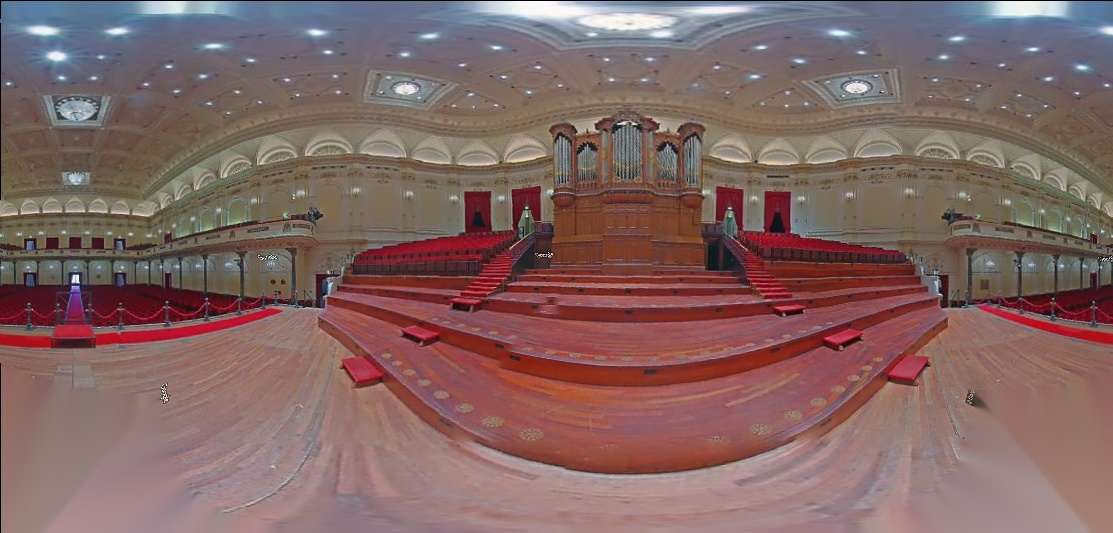
\includegraphics[width=5cm]{images/google_example/original}
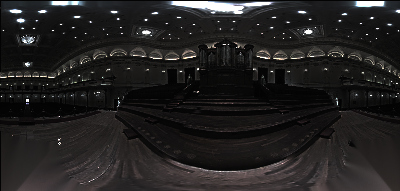
\includegraphics[width=5cm]{images/google_example/dark}
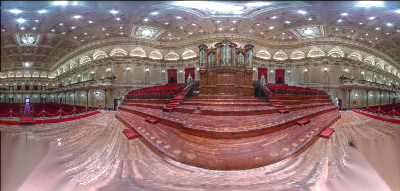
\includegraphics[width=5cm]{images/google_example/bright}
\caption{An example LDR panorama, with dark and light exposures extracted the predicted HDR environment.}\label{fig:google}
Source: Google
\end{figure}
\subsection{Bootstrapping Extra Light Probes}
A significant issue with generating the data is the lack of large datasets of HDRI environment maps. We initially used a dataset of 175 environment maps from HDRIHaven.com, an improvement over the 105 in \cite{RematasCVPR2016}. We found that our validation scores on unseen lighting continued to improve indicating that our model was not overfitting to the lighting scenarios presented. Qualitatively however it appeared that the model would primarily learn features from the training lightmaps and was at times effectively selecting the closest previously seen environment. This could be confirmed by training a model without the background present, which would perform significantly worse. While this may be effective at producing realistic lighting, the aim of this work is to encourage the model to learn how the reflectance of an object maps to the lighting conditions. To mitigate this behaviour and reduce overfitting to the environment we aimed to increase the size of our lighting dataset considerably. 
\newline
Collecting additional HDRI panoramas would be infeasible due to the lack of equipment and time and so we took the approach to producing HDR estimates from existing LDR content. The biggest available dataset of LDR panoramas is Google Street View \cite{GoogleMaps}, with both indoor and outdoor scenes. While this dataset is huge and provides a more realistic sample of lighting conditions, it is only available in low dynamic range. Fortunately, there is plenty of previous work in the area of converting LDR content to HDR, particularly using CNNS to find light sources and tonemap content. We make use of \cite{2018arXiv180302266M}, a very recent work that uses both a local and global branches to produce accurate tonemappng predictions. It is important to note that this network is intended as a general purpose image regressor, and is not trained on panoramas in particular. It would certainly be possible to improve results by retraining, or fine-tuning, the network on our existing set of HDR panoramas to produce better light probes. We make use of the image stitching and inpainting tools within OpenCV to create panoramas from different views on Google Street View, and use the aforementioned HDR-Expandnet to bolster our dataset with an additional 237 lightmaps. An example is shown in \ref{fig:google} Our models are trained both with and without these additions to find any issues with overfitting or malformed data produced by ExpandNet.
\begin{figure}[H]
\centering
\includegraphics[height=10cm]{images/Stereo}
\caption 
\newline
The first stereo image architecture. Weights are shared in the first 3 encode blocks, and the outputs are simply concatenated.
\label{basic}
\end{figure}
\section{Model Architecture}
\subsection{Siamese Layers}
To construct a model that produces good results, while minimising network size for performance and training times, it is important to carefully consider the problem being solved and the features and patterns that are being learned. By using stereo views we aim to find correspondance between similar features and an understanding of geometry due to the parallax effect. To this end we present results from a 'siamese' network, where the weights in the convolutional layers are shared, such that the same features are extracted from each view. The two inputs are fed into two identical 'Encode' blocks, consisting of a number of convolutional layers with batch normalization and max pooling. However, during the training process, only the weights for the first path are trained. These weights are duplicated in the second path to ensure that the same convolutions are being performed on each image of the pair. The output of these two paths is then concatenated before being passed into the deconvolutional steps, as shown in \ref{basic}. We make use of \textit{Skip Connections}, which have been shown to improve the performance of similar image regression networks such as \textit{Pix2Pix} \cite{DBLP:journals/corr/IsolaZZE16}.
\newline
\subsection{Cosine Similarity Pyramid}
\begin{figure}[H]
\label{pyramid}
\centering
\includegraphics[width=14cm]{images/Pyramid}
\caption{The Cosine SImilarity Pyramid as implemented. Decode path removed for brevity.}
\end{figure}
We can further encourage the network to perform stereo matching by using the dot product technique as suggested in \cite{7780983}. After using shared weights to extract the same features from each image, we then perform a dot product operation on the L2-Normalised output to find the \textit{Cosine Similarity}
\[\bm{a}\cdot \bm{b} = \lvert a \rvert \lvert b\rvert \cos(\theta) \]
which represents the cosine of the angle between the two inputs. On a raw image, if two pixels are identical in value, they will have a cosine similarity of 1, and so we would find the nearest matching points from the values closest to 1. Instead of comparing raw pixels, we instead compare the intermediate representation, to find the similarity between features rather than pixels. The resultant correlations then represent the feature disparity maps. The correlation can then be concatenated with the original features before being passed as input to further convolutional layers, starting with a 1x1 convolution to act as a \textit{Fusion} layer.
\newline
A drawback of traditional block-disparity methods for stereo matching is that the block size significantly affects the accuracy of the calculated disparity. Larger block sizes have the important benefit of reliability, as it is easier to find unique matching blocks within the two images than it is to find matching pixels, for example. In our \textit{Cosine Similarity} step, we are effectively performing a block disparity on a spatially reduced representation of the image. Industry standard stereo matching methods deal with this by using a pyramid of block sizes, and fusing the results. To avoid suffering the same problems, we present a different model using a \textit{Cosine Similarity Pyramid}, where we perform our similarity step of each intermediate stereo output, as shown in \ref{pyramid}. This way, we can estimate similarity of features at different scales, exploting both the robustness of large blocks and the accuracy of small ones. Each similarity is concatenated to the stereo output as before. This method does present a significant performance comprimise, requiring more computation and memory to produce our full intermediate similarity representation.
\subsection{Training Details}
 We experimented with different model parameters to achieve thr best validation accuracies. For each architecture, we varied the number of convolutional layers per encode-block, making it easier to test different model depths without major changes to teh codebase. We discovered early on that deeper models consistently perform better than their shallow counterparts, but somewhat mitigate the benefits of our cosine similarity steps. However it is important to consider the computational performance of the result and so we test all architectures at a range of depths.
\newline
The original Dematerial network was trained with a \textit{Gradient Descent} optimizer, using a momentum on the learning rate such that it decreases over time. The idea is that the learning rate decreases as the model reaches the optimum, to fine-tune the weightings. We found that we could achieve faster training using the ADAM optimiser, which maintains a per-parameter learning rate using the second moments of the gradients after loss calculation to produce new weights. We were also able to use a higher learning rate of 1.7e-5. Often the performance of details such as these are very dependent on implementation details like the framework used or the hardware being trained on. As a result our choice to make these changes is not alone an indication that the previous work could be improved in the same way.
\newline
Our deep model uses 9 convolutional layers per input branch, 9 convolutional layers for branch fusion and 9 more to produce the environment map. In comparison the original Dematerial network used 13 convolutional layers per branch, and 15 to produce the environment map. To evaluate our new model features we experiment with different model depths.
\newline
For our prediction task we make the following assumptions:
\begin{itemize}
\item Provided objects consist of a single material with constant albedo. Materials can contain Diffuse, Specular and Subsurface properties.
\item Geometry and lighting remain static between both stereo views.
\item Stereo view distance is kept constant, though object size can vary. Views are also parallel, and images are not manually rectified.
\item Subjects are modelled as floating objects. In the use-case where lighting on a surface is required, the surface lighting can be composited onto the light probe trivially.
\item Camera intrinsics are kept constant.
\end{itemize}

\section{Experiments}
To determine the best features for the task, we evaluated the performance of a suite of configurations:
\begin{itemize}
\item Dematerial model with known geometry.
\item Basic Concatenation model without shared weights.
\item Basic Concatenation model with shared weights.
\item Single Dot Product model.
\item Single Dot Product model without background data.
\item Single Dot Product model with augmented data.
\item Cosine Similarity Pyramid model.
\item Cosine Similarity Pyramid model with Multi-Scale features.
\end{itemize}
All models were trained for 100 epochs, with a learning rate of 1.7e-8, and evaluated on 1000 validation samples. A batch size of only 24 was used, due to memory requirements of the larger networks. We only quanititatively evaulate the quality of the lighting prediction, however surface normals are also produced as an output too all models aside from 'Dematerial'.
\chapter{Critical Evaluation}
\label{chap:evaluation}
\section{Experimental Results}
\subsection{Effect of Shared Weights}
\begin{figure}[H]
\newlength\figureheight
\newlength\figurewidth
\setlength\figureheight{6cm}
\setlength\figurewidth{12cm}
\centering
% This file was created by matplotlib2tikz v0.6.16.
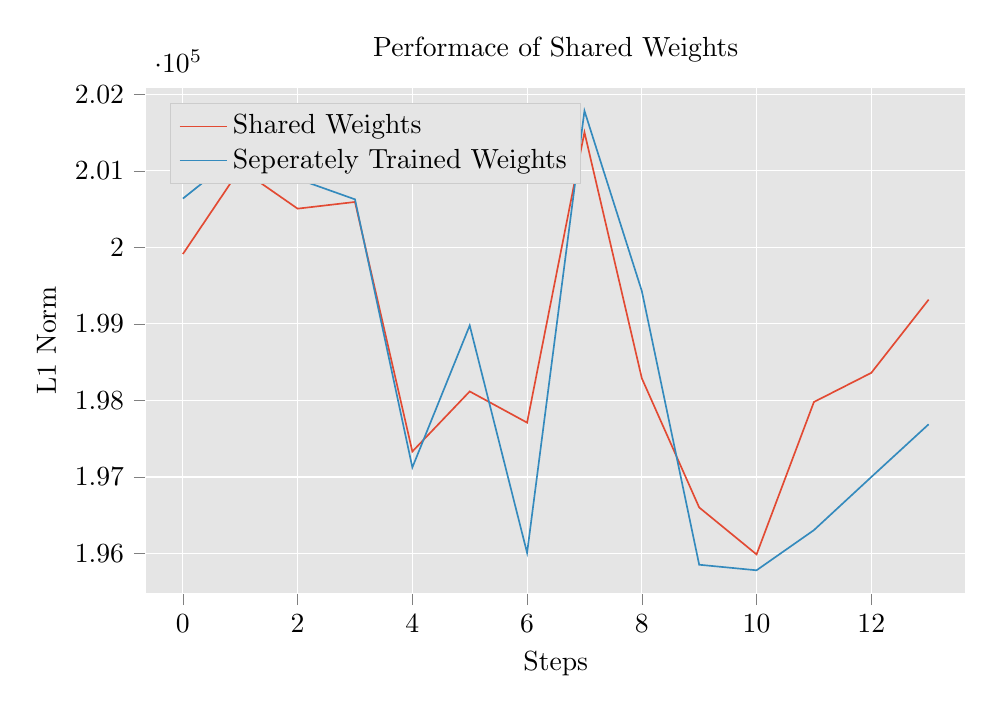
\begin{tikzpicture}

\definecolor{color1}{rgb}{0.203921568627451,0.541176470588235,0.741176470588235}
\definecolor{color0}{rgb}{0.886274509803922,0.290196078431373,0.2}

\begin{axis}[
title={Performace of Shared Weights},
xlabel={Steps},
ylabel={L1 Norm},
xmin=-0.65, xmax=13.65,
ymin=195480.29140625, ymax=202083.84921875,
width=12cm,
height=8cm,
tick align=outside,
tick pos=left,
xmajorgrids,
x grid style={white},
ymajorgrids,
y grid style={white},
axis line style={white},
axis background/.style={fill=white!89.80392156862746!black},
legend entries={{Shared Weights},{Seperately Trained Weights}},
legend style={at={(0.03,0.97)}, anchor=north west, draw=white!80.0!black, fill=white!89.80392156862746!black},
legend cell align={left}
]
\addlegendimage{no markers, color0}
\addlegendimage{no markers, color1}
\addplot [semithick, color0]
table {%
0 199912.765625
1 201026.984375
2 200505.734375
3 200593.0625
4 197332.296875
5 198117.484375
6 197710.078125
7 201504.21875
8 198289.265625
9 196601.453125
10 195987.859375
11 197979.546875
12 198360.421875
13 199317.171875
};
\addplot [semithick, color1]
table {%
0 200637.09375
1 201236.375
2 200893.953125
3 200627.1875
4 197124.421875
5 198979.375
6 196008.40625
7 201783.6875
8 199429.421875
9 195853.15625
10 195780.453125
11 196305.421875
12 196999.203125
13 197688.421875
};
\end{axis}

\end{tikzpicture}
\caption{SSD between the predicted lighting and ground truth on the validation set, at each epoch during the training process. In both models, 3 Convolutions are used for each Encode/Decode block, and the outputs of the stereo branches are concatenated.}
\end{figure}
We found that using shared weights on our basic concatenation model had very little effect on the accuracy of results. In our training process we use the L1 norm loss to determine how to reweight our graph. For the siamese network, new weights are only calculated for the left branch, and then duplicated to the right branch. When the weights are trained seperately, they will eventually converge on, or even outperform the original weightings.
\subsection{Concatenation VS Dot Product}
\begin{figure}[H]
\setlength\figureheight{6cm}
\setlength\figurewidth{12cm}
\centering
% This file was created by matplotlib2tikz v0.6.16.
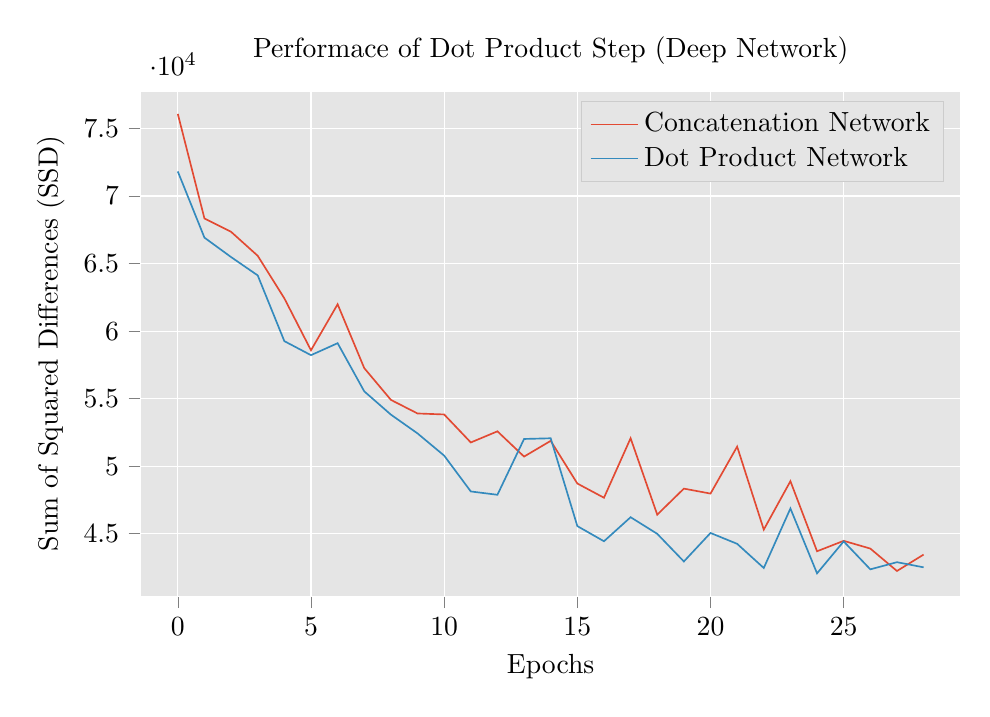
\begin{tikzpicture}

\definecolor{color1}{rgb}{0.203921568627451,0.541176470588235,0.741176470588235}
\definecolor{color0}{rgb}{0.886274509803922,0.290196078431373,0.2}

\begin{axis}[
title={Performace of Dot Product Step (Deep Network)},
xlabel={Epochs},
ylabel={Sum of Squared Differences (SSD)},
xmin=-1.4, xmax=29.4,
ymin=40366.170703125, ymax=77775.477734375,
width=12cm,
height=8cm,
tick align=outside,
tick pos=left,
xmajorgrids,
x grid style={white},
ymajorgrids,
y grid style={white},
axis line style={white},
axis background/.style={fill=white!89.80392156862746!black},
legend entries={{Concatenation Network},{Dot Product Network}},
legend style={draw=white!80.0!black, fill=white!89.80392156862746!black},
legend cell align={left}
]
\addlegendimage{no markers, color0}
\addlegendimage{no markers, color1}
\addplot [semithick, color0]
table {%
0 76075.0546875
1 68337.9921875
2 67347.7265625
3 65573.9296875
4 62423.07421875
5 58579.0625
6 61986.05859375
7 57258.51171875
8 54909.62890625
9 53902.23828125
10 53829.10546875
11 51756.33203125
12 52581.04296875
13 50711.17578125
14 51876.11328125
15 48717.28515625
16 47665.23828125
17 52069.20703125
18 46413.140625
19 48339.9375
20 47972.359375
21 51450.33203125
22 45306.125
23 48890.04296875
24 43702.51171875
25 44475.0625
26 43902.12890625
27 42242.75390625
28 43456.56640625
};
\addplot [semithick, color1]
table {%
0 71815.9140625
1 66918.078125
2 65479.265625
3 64121.98046875
4 59256.625
5 58217.87890625
6 59104.46875
7 55539.98828125
8 53817.453125
9 52427.26953125
10 50782.52734375
11 48130.453125
12 47883.140625
13 52014.94921875
14 52066.69140625
15 45566.328125
16 44443.25390625
17 46223.32421875
18 44993.12890625
19 42946.69140625
20 45057.19140625
21 44253.609375
22 42463.171875
23 46869.61328125
24 42066.59375
25 44432.17578125
26 42364.625
27 42895.50390625
28 42513.109375
};
\end{axis}

\end{tikzpicture}
\caption{SSD between the predicted lighting and ground truth on the validation set, at each epoch during the training process. In the first model, the outputs from the stereo branches are concatenated, in the other we use normalisation and dot product to determine Cosine Similarity. Both models use 3 layers per block.}
\end{figure}
The dot product step results in a small improvement in accuraccy and a significant improvement in training speed. The dot product step is effectively a manually calculated similarity measure between the two views, and so the model can converge on the depth features earlier in the training process. We believe that the performance difference is minimal as the model is already very deep, and training would likely converge on the depth features eventually.
As a result we also show the effect with a much shallower model.
\begin{figure}[H]
\setlength\figureheight{6cm}
\setlength\figurewidth{12cm}
\centering
% This file was created by matplotlib2tikz v0.6.16.
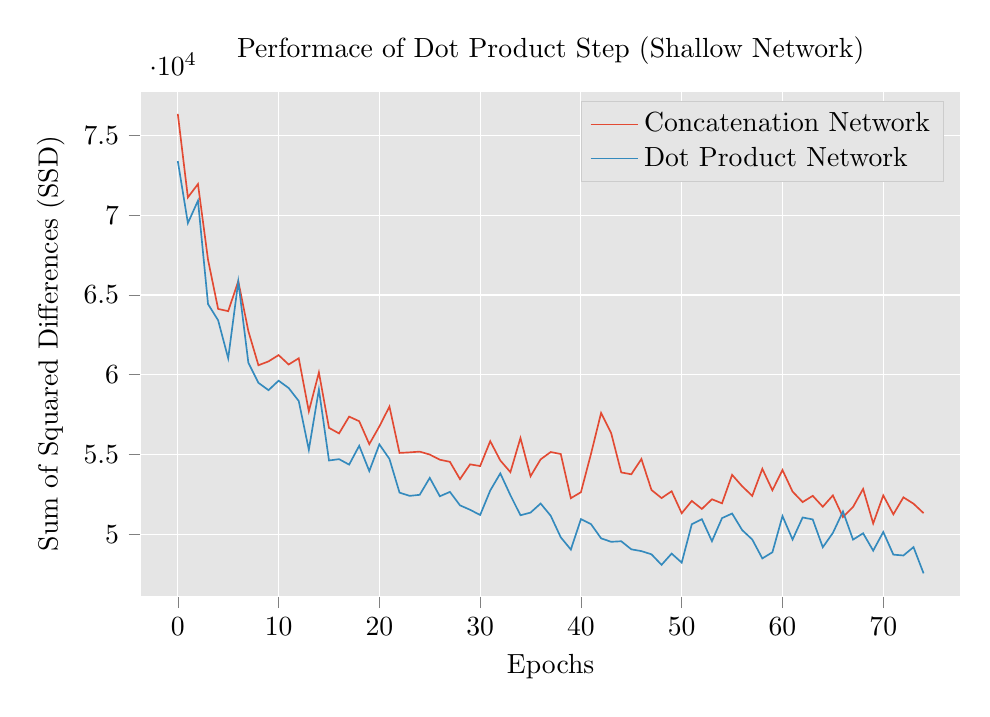
\begin{tikzpicture}

\definecolor{color1}{rgb}{0.203921568627451,0.541176470588235,0.741176470588235}
\definecolor{color0}{rgb}{0.886274509803922,0.290196078431373,0.2}

\begin{axis}[
title={Performace of Dot Product Step (Shallow Network)},
xlabel={Epochs},
ylabel={Sum of Squared Differences (SSD)},
xmin=-3.7, xmax=77.7,
ymin=46100.3080078125, ymax=77792.5240234375,
width=12cm,
height=8cm,
tick align=outside,
tick pos=left,
xmajorgrids,
x grid style={white},
ymajorgrids,
y grid style={white},
axis line style={white},
axis background/.style={fill=white!89.80392156862746!black},
legend entries={{Concatenation Network},{Dot Product Network}},
legend style={draw=white!80.0!black, fill=white!89.80392156862746!black},
legend cell align={left}
]
\addlegendimage{no markers, color0}
\addlegendimage{no markers, color1}
\addplot [semithick, color0]
table {%
0 76351.96875
1 71117.0546875
2 71955.4609375
3 67205.3203125
4 64124.5625
5 63982.953125
6 65862.359375
7 62730.09765625
8 60590.8125
9 60832.90625
10 61228.30859375
11 60637.75
12 61030.08984375
13 57703.96875
14 60139.66796875
15 56665.75390625
16 56316.37109375
17 57370.06640625
18 57081.84375
19 55645.140625
20 56757.48828125
21 57998.80078125
22 55093.46484375
23 55129.10546875
24 55174.828125
25 54991.52734375
26 54667.546875
27 54535.46484375
28 53449.65625
29 54377.41015625
30 54269.484375
31 55830.96484375
32 54619.46875
33 53889.08203125
34 56029.55078125
35 53631.953125
36 54689.28515625
37 55150.22265625
38 55024.390625
39 52253.77734375
40 52631.890625
41 55037.73828125
42 57601.19140625
43 56334.703125
44 53869.78125
45 53753.93359375
46 54711.68359375
47 52770.390625
48 52262.109375
49 52690.29296875
50 51312.76953125
51 52084.48828125
52 51580.90234375
53 52188.34765625
54 51933.05859375
55 53719.30078125
56 53002.00390625
57 52400.02734375
58 54097.60546875
59 52750.41015625
60 54018.41015625
61 52669.06640625
62 52010.19140625
63 52403.515625
64 51717.859375
65 52430.33984375
66 51069.22265625
67 51704.84375
68 52835.58203125
69 50671.625
70 52429.33203125
71 51243.26953125
72 52308.34375
73 51909.51171875
74 51317.17578125
};
\addplot [semithick, color1]
table {%
0 73394.546875
1 69506.5234375
2 70909.7890625
3 64425.296875
4 63411.30078125
5 61028.50390625
6 65840.78125
7 60750.09375
8 59488.41796875
9 59028.65234375
10 59623.71875
11 59163.08203125
12 58349.31640625
13 55292.046875
14 59072.578125
15 54618.953125
16 54703.67578125
17 54359.640625
18 55541.76171875
19 53957.76171875
20 55630.640625
21 54717.109375
22 52605.16796875
23 52400.73046875
24 52465.71484375
25 53529.859375
26 52373.50390625
27 52651.0625
28 51805.91015625
29 51528.87890625
30 51200.26953125
31 52736.30859375
32 53810.796875
33 52444.37890625
34 51184.08203125
35 51351.953125
36 51920.33984375
37 51156.234375
38 49801.25390625
39 49032.63671875
40 50942.35546875
41 50627.05078125
42 49738.62109375
43 49519.57421875
44 49555.26953125
45 49047.65234375
46 48936.09765625
47 48735.796875
48 48074.16796875
49 48781.09765625
50 48215.35546875
51 50621.68359375
52 50941.546875
53 49557.98828125
54 51005.703125
55 51293.96484375
56 50254.953125
57 49663.81640625
58 48477.23828125
59 48866.15234375
60 51133.48828125
61 49662.11328125
62 51046.66015625
63 50923.33203125
64 49177.34375
65 50078.453125
66 51422.77734375
67 49656.375
68 50053.5625
69 48965.765625
70 50135.90625
71 48715.640625
72 48661.94140625
73 49186.546875
74 47540.86328125
};
\end{axis}

\end{tikzpicture}
\caption{In the first model, the outputs from the stereo branches are concatenated, in the other we use normalisation and dot product to determine Cosine Similarity. Both models use 1 convolutional layer per block.}
\end{figure}
The shallow model uses 1 Convolutional layer per Encode block, resulting in 3 convolutional layers per stereo branch, 3 more for branch fusion, and 3 to produce the lighting. The memory requirements for this graph much lower than the deep model, but the performance is very similar. Here we can see a consistent, although modest, improvement in performance from using the Cosine Similarity. We believe a limiting factor in this approach for lighting estimation is that many differences in stereo views are not due to the relative movement of geometry relied upon for depth calculation. For example, specularity depends heavily on view direction. By performing the dot product we are treating these features the same as geometric features.
\newline
Another issue with this is that we are also performing the dot product on features extracted from the background. In our case the background is modelled to be infinitely far away, and while it contains useful contextual and hue information, should not be used in the similarity measure.
\subsection{Effect of Background}
\begin{figure}[H]
\setlength\figureheight{6cm}
\setlength\figurewidth{12cm}
\centering
% This file was created by matplotlib2tikz v0.6.16.
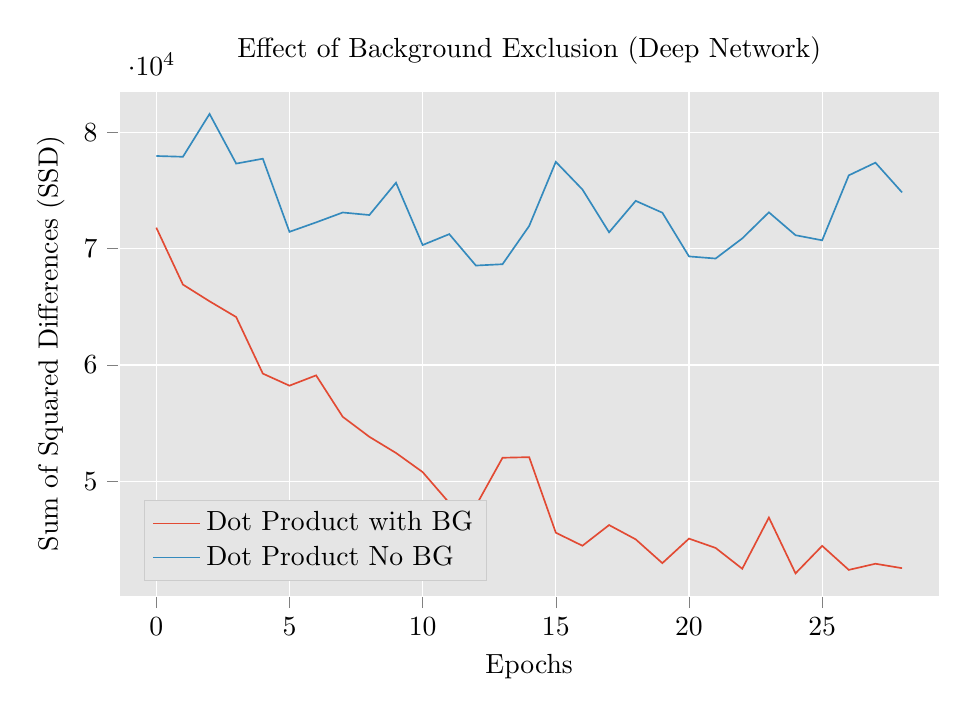
\begin{tikzpicture}

\definecolor{color1}{rgb}{0.203921568627451,0.541176470588235,0.741176470588235}
\definecolor{color0}{rgb}{0.886274509803922,0.290196078431373,0.2}

\begin{axis}[
title={Effect of Background Exclusion (Deep Network)},
xlabel={Epochs},
ylabel={Sum of Squared Differences (SSD)},
xmin=-1.4, xmax=29.4,
ymin=40089.8203125, ymax=83578.8359375,
width=12cm,
height=8cm,
tick align=outside,
tick pos=left,
xmajorgrids,
x grid style={white},
ymajorgrids,
y grid style={white},
axis line style={white},
axis background/.style={fill=white!89.80392156862746!black},
legend style={at={(0.03,0.03)}, anchor=south west, draw=white!80.0!black, fill=white!89.80392156862746!black},
legend cell align={left},
legend entries={{Dot Product with BG},{Dot Product No BG}}
]
\addlegendimage{no markers, color0}
\addlegendimage{no markers, color1}
\addplot [semithick, color0]
table {%
0 71815.9140625
1 66918.078125
2 65479.265625
3 64121.98046875
4 59256.625
5 58217.87890625
6 59104.46875
7 55539.98828125
8 53817.453125
9 52427.26953125
10 50782.52734375
11 48130.453125
12 47883.140625
13 52014.94921875
14 52066.69140625
15 45566.328125
16 44443.25390625
17 46223.32421875
18 44993.12890625
19 42946.69140625
20 45057.19140625
21 44253.609375
22 42463.171875
23 46869.61328125
24 42066.59375
25 44432.17578125
26 42364.625
27 42895.50390625
28 42513.109375
};
\addplot [semithick, color1]
table {%
0 77981.546875
1 77914.5078125
2 81602.0625
3 77327.15625
4 77749.1640625
5 71455.625
6 72268.7109375
7 73119.2734375
8 72902.3203125
9 75683.4921875
10 70319.9375
11 71257.7265625
12 68554.953125
13 68669.1015625
14 71960.2578125
15 77478.421875
16 75098.2890625
17 71414.4453125
18 74120.765625
19 73100.7265625
20 69340.5390625
21 69158.5390625
22 70889.375
23 73134.9296875
24 71164.2421875
25 70725.546875
26 76315.390625
27 77407.84375
28 74847.6796875
};
\end{axis}

\end{tikzpicture}
\caption{In the first model, the object is composited onto the background, while in the second model, the background is not present and replaced with 0 values.}
\end{figure}
The model is able to infer some of the lighting without the background, indicating that it is learning the lighting conditions from the subject. However, adding the background improves the performance significantly. The background not only gives an indication of the physical environment the subject inhabits, but also the colors and intensities to expect. This data, in theory, should make it easier to determine the difference between reflectance, albedo and shadows on the subject as well as indicate the hue of the resulting environment map. Our results indicate that the background information is useful for estimating the lighting accurately. For a robust model we cannot exclude the background, however it cannot be included in our Cosine Similarity steps. To solve this we present a new network where the background is given it's own branch.
\begin{figure}[H]
\setlength\figureheight{6cm}
\setlength\figurewidth{12cm}
\centering
% This file was created by matplotlib2tikz v0.6.16.
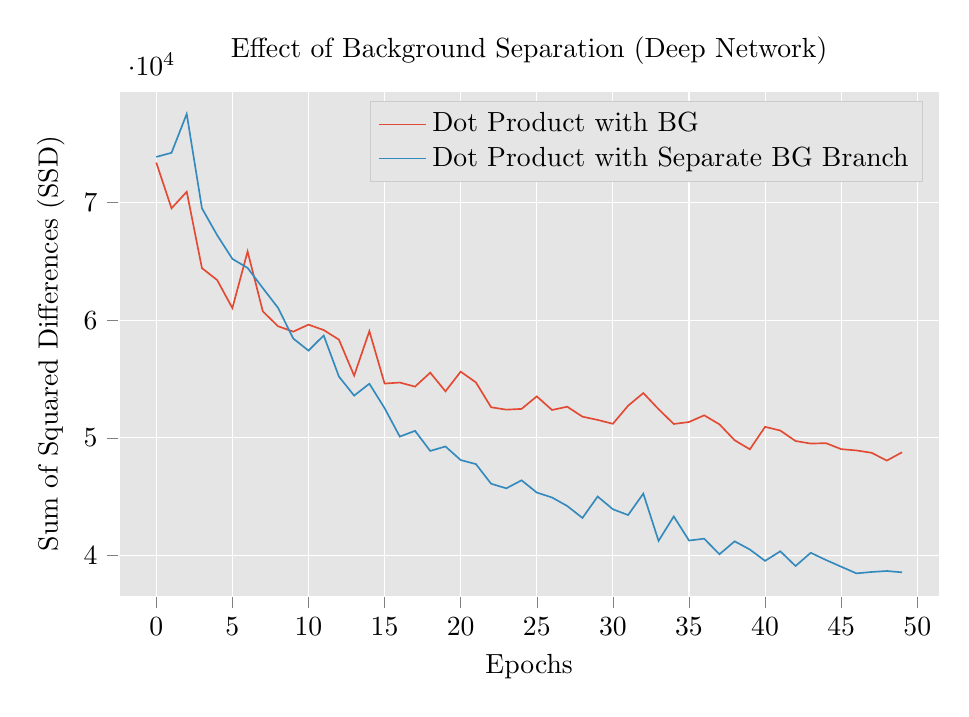
\begin{tikzpicture}

\definecolor{color1}{rgb}{0.203921568627451,0.541176470588235,0.741176470588235}
\definecolor{color0}{rgb}{0.886274509803922,0.290196078431373,0.2}

\begin{axis}[
title={Effect of Background Separation (Deep Network)},
xlabel={Epochs},
ylabel={Sum of Squared Differences (SSD)},
xmin=-2.45, xmax=51.45,
ymin=36542.38125, ymax=79475.93125,
width=12cm,
height=8cm,
tick align=outside,
tick pos=left,
xmajorgrids,
x grid style={white},
ymajorgrids,
y grid style={white},
axis line style={white},
axis background/.style={fill=white!89.80392156862746!black},
legend style={draw=white!80.0!black, fill=white!89.80392156862746!black},
legend entries={{Dot Product with BG},{Dot Product with Separate BG Branch}},
legend cell align={left}
]
\addlegendimage{no markers, color0}
\addlegendimage{no markers, color1}
\addplot [semithick, color0]
table {%
0 73394.546875
1 69506.5234375
2 70909.7890625
3 64425.296875
4 63411.30078125
5 61028.50390625
6 65840.78125
7 60750.09375
8 59488.41796875
9 59028.65234375
10 59623.71875
11 59163.08203125
12 58349.31640625
13 55292.046875
14 59072.578125
15 54618.953125
16 54703.67578125
17 54359.640625
18 55541.76171875
19 53957.76171875
20 55630.640625
21 54717.109375
22 52605.16796875
23 52400.73046875
24 52465.71484375
25 53529.859375
26 52373.50390625
27 52651.0625
28 51805.91015625
29 51528.87890625
30 51200.26953125
31 52736.30859375
32 53810.796875
33 52444.37890625
34 51184.08203125
35 51351.953125
36 51920.33984375
37 51156.234375
38 49801.25390625
39 49032.63671875
40 50942.35546875
41 50627.05078125
42 49738.62109375
43 49519.57421875
44 49555.26953125
45 49047.65234375
46 48936.09765625
47 48735.796875
48 48074.16796875
49 48781.09765625
};
\addplot [semithick, color1]
table {%
0 73874.3203125
1 74221.1484375
2 77524.40625
3 69507.4375
4 67222.1484375
5 65208.41015625
6 64442.390625
7 62727.33203125
8 61050.625
9 58442.234375
10 57418.35546875
11 58700.74609375
12 55213.953125
13 53593.765625
14 54604.19140625
15 52530.640625
16 50110.39453125
17 50601.37890625
18 48894.015625
19 49275.03125
20 48117.859375
21 47777.48828125
22 46107.5625
23 45716.95703125
24 46400.52734375
25 45357.85546875
26 44942.390625
27 44216.6875
28 43201.11328125
29 45023.23828125
30 43940.234375
31 43448.9765625
32 45269.16796875
33 41254.00390625
34 43331.609375
35 41284.3828125
36 41438.10546875
37 40116.984375
38 41215.10546875
39 40519.515625
40 39557.375
41 40369.86328125
42 39119.04296875
43 40241.8046875
44 39629.44921875
45 39058.53515625
46 38493.90625
47 38612.125
48 38694.61328125
49 38581.05859375
};
\end{axis}

\end{tikzpicture}
\caption{In the first model, the object is composited onto the background, while in the second model, the object is provided on a 0 value background, while the real background is provided to a different branch. The output of this branch is concatenated to the dot product output.}
\end{figure}
A separate background, as used by the Dematerial network, results in significant improvements over our original network. In fact, the shallow network now outperforms the deeper networks that didn't include our augmentations.


\subsection{Cosine Similarity Pyramid}
\begin{figure}[H]
\setlength\figureheight{6cm}
\setlength\figurewidth{12cm}
\centering
% This file was created by matplotlib2tikz v0.6.16.
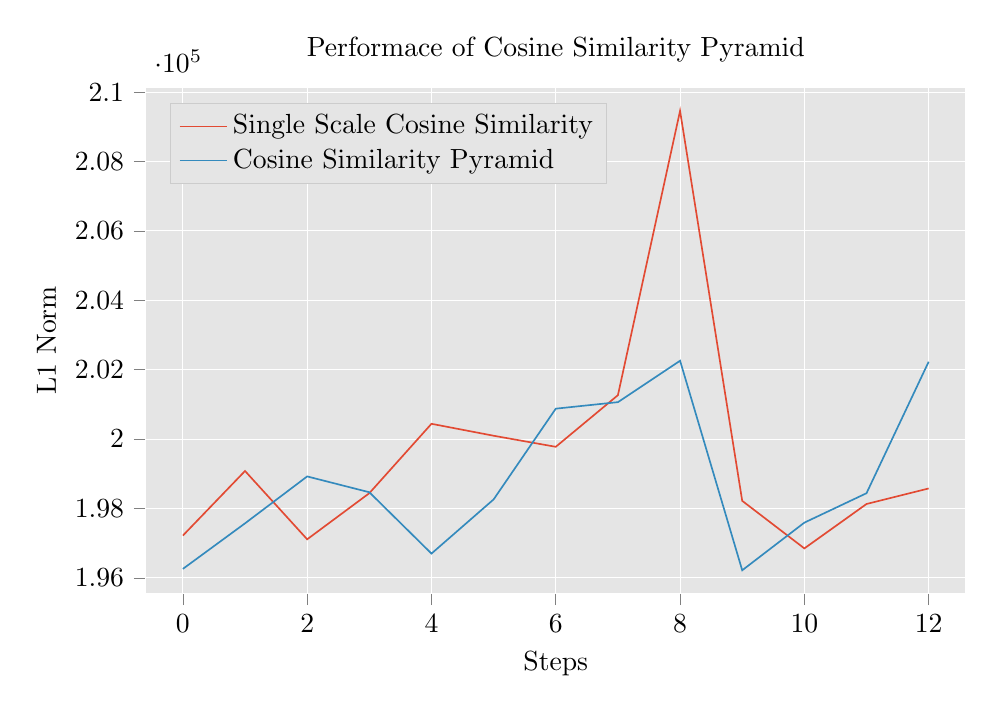
\begin{tikzpicture}

\definecolor{color1}{rgb}{0.203921568627451,0.541176470588235,0.741176470588235}
\definecolor{color0}{rgb}{0.886274509803922,0.290196078431373,0.2}

\begin{axis}[
title={Performace of Cosine Similarity Pyramid},
xlabel={Steps},
ylabel={L1 Norm},
xmin=-0.6, xmax=12.6,
ymin=195555.86015625, ymax=210121.56171875,
width=12cm,
height=8cm,
tick align=outside,
tick pos=left,
xmajorgrids,
x grid style={white},
ymajorgrids,
y grid style={white},
axis line style={white},
axis background/.style={fill=white!89.80392156862746!black},
legend entries={{Single Scale Cosine Similarity},{Cosine Similarity Pyramid}},
legend style={at={(0.03,0.97)}, anchor=north west, draw=white!80.0!black, fill=white!89.80392156862746!black},
legend cell align={left}
]
\addlegendimage{no markers, color0}
\addlegendimage{no markers, color1}
\addplot [semithick, color0]
table {%
0 197218.3125
1 199080.0625
2 197110.71875
3 198440.03125
4 200439.765625
5 200095.78125
6 199776.78125
7 201264.515625
8 209459.484375
9 198219.90625
10 196848.78125
11 198128.296875
12 198576.578125
};
\addplot [semithick, color1]
table {%
0 196258.0625
1 197571.0625
2 198923.0625
3 198467.046875
4 196699.53125
5 198260.65625
6 200876.03125
7 201064.0625
8 202257.921875
9 196217.9375
10 197591.296875
11 198439.125
12 202228.28125
};
\end{axis}

\end{tikzpicture}
\caption{Comparison of model with single Similarity layer, and model with a pyramid of similarity measurements.}
\end{figure}
With the gain in performance from performing a Cosine Similarity on the stereo branch output, we expected that we could gain additional performance by finding similarities at a range of layer depths. In theory, we would find the feature similarity across receptive field sizes, giving more depth information to the fusion network. However we found this had little effect on accuracy. We believe that the features are uneccesary at the scale provided - that of a single floating nearby object. In more complex scenarios, such as depth inference across a full scene, finding similarity at a range of receptive field sizes may use useful. Furthermore if the features are useful, the fusion network would need to be deeper to extract the useful information.
\section{Final Model Accuracy}
\subsection{Metrics}
From our experiments we determined to choose our shallow stereo model, with a seperated background and a cosine similarity block as our final model for evaluation. To evaluate the accuracy of the model we use a suite of image comparison measures on the produced HDRI environment maps. It is essential that the metrics used suitably evaulate the image similarity, and so we consider which image properties are most influential of the resulting lighting. The most basic estimation should be able to capture the direction and intensity of direct lights within the scene. Often there are few direct lights, but their effect on lighting dominates the overall scene illumination. Better predictions will be able to capture some information on indirect lighting, such as sky or wall colour and brightness.
\newline 
We start with two basic difference metrics, the L1 norm and L2 norm, which are both per-pixel Minkowski distances. These measures are fast to calculate and simple to implement and so are often used as the loss function in image regression tasks. L2 norm, also cannel \textit{Mean Squared Error}, involves the squaring of pixel differences, and exagerrates the effect of large pixel differences on the overall similarity score. In the HDR domain this can mean that direct lights, such as the sun, which are predicted to be in a slightly different direction, will have a severe impact on the similarity, despite having a minor effect on the resulting illumination. When we inspect light sources in sRGB photographs, it appears as if the light source is large and emmitting light from a radius, as the higher brightness values fall outside of the cameras exposure bracket. \ref{rgb_example} demonstrates this effect, as parts of the woman's face, as well as the surrounding sky have the same colour values as the center of the sun, as the camera fails to capture the brightness rage. A minor misprediction in sun position here will have little effect on the L2 distance, but in HDR would have a significant impact. 
\newline
Another commonly used image comparison metric is the SSIM \cite{1284395},
\[SSIM(x,y) = \frac{(2u_xu_y + c_1)(2\sigma_{xy} + c_2)}{(u^2_x + u^2_y + c_1)(\sigma^2_x + \sigma^2_y + c_2)}\]
which aims to predict the accuracy of an image with human perception. It is a measure of structure, which takes luminance and contrast into account, and so is better suited for HDR. Finally, we assess the models ability to identify the direction of the provailing light source, by taking the distance between the brightest pixel in the ground truth and predicted image. For assessment we use a validation set of 1000 images, under new environment maps and models with random materials and rotations.
\subsection{Results}
On our synthetic benchmark, our stereo model achieved a Mean Squared Error of 1134.83, with the 50th and 75th percentile being 2.17 and 7.62 respectively. This implies that while the model performs well in most tested scenarios, there are some cases where the predictions are vastly incorrect, as shown in \ref{mse_results}. It is also clear from the qualitative results that the MSE is not the ideal metric in our case. While it favours structure and sky location, it seems to fail to capture the primary light direction. As a result, renders produced with the best MSE results tend to have good environment lighting, but completely incorrect shadowing due to a failure to predict direct lighting.
\newline
\begin{figure}[H]
\centering
\begin{tabular}{ |p{3cm}||p{3cm}|p{3cm}|p{3cm}|p{3cm}|  }
 \hline
 \multicolumn{5}{|c|}{MSE Evaluation} \\
 \hline
  & Input Data &Ground Truth Environment&Predicted Environment&MSE Score\\
 \hline
 25th Percentile(Synth)&\parbox[c]{1em}{
 \includegraphics[width=2cm,trim=-10 0 0 -10]{images/deep_stereo/25p_mse_input}}&\parbox[c]{1em}{\includegraphics[width=2cm,trim=-10 0 0 -10]{images/deep_stereo/25p_mse_gt_tm}}&
\parbox[c]{1em}{\includegraphics[width=2cm,trim=-10 0 0 -10]{images/deep_stereo/25p_mse_pred_tm}}& 0.22\\
 50th Percentile(Synth)&\parbox[c]{1em}{
 \includegraphics[width=2cm,trim=-10 0 0 -10]{images/deep_stereo/50p_mse_input}}&\parbox[c]{1em}{\includegraphics[width=2cm,trim=-10 0 0 -10]{images/deep_stereo/50p_mse_gt_tm}}&
\parbox[c]{1em}{\includegraphics[width=2cm,trim=-10 0 0 -10]{images/deep_stereo/50p_mse_pred_tm}}& 0.30\\
 75th Percentile(Synth)&\parbox[c]{1em}{
 \includegraphics[width=2cm,trim=-10 0 0 -10]{images/deep_stereo/75p_mse_input}}&\parbox[c]{1em}{\includegraphics[width=2cm,trim=-10 0 0 -10]{images/deep_stereo/75p_mse_gt_tm}}&
\parbox[c]{1em}{\includegraphics[width=2cm,trim=-10 0 0 -10]{images/deep_stereo/75p_mse_pred_tm}}& 0.41\\
 \hline
\end{tabular}

\label{mse_results}
\caption{Demonstration on test set.}

\end{figure}
For the SSIM test, the stereo model achieves a respectable average of 0.28, with 50th and 75th percentiles of 0.28 and 0.35. Here the spread of results is much tighter, and we can see from \ref{ssim_results} that the metric captures the structure of the environment very well. These results are better than many of the models of Georgoulis et al. \cite{Georgoulis_2017_ICCV}, which all rely on known geometry.
  \todo{Little table here}
 \newline
 \begin{figure}[H]
\centering
\begin{tabular}{ |p{3cm}||p{3cm}|p{3cm}|p{3cm}|p{3cm}|  }
 \hline
 \multicolumn{5}{|c|}{SSIM Evaluation} \\
 \hline
  & Input Data &Ground Truth Environment&Predicted Environment&SSIM Score\\
 \hline
 25th Percentile(Synth)&\parbox[c]{1em}{
 \includegraphics[width=2cm,trim=-10 0 0 -10]{images/deep_stereo/25p_ssim_input}}&\parbox[c]{1em}{\includegraphics[width=2cm,trim=-10 0 0 -10]{images/deep_stereo/25p_ssim_gt_tm}}&
\parbox[c]{1em}{\includegraphics[width=2cm,trim=-10 0 0 -10]{images/deep_stereo/25p_ssim_pred_tm}}& 0.22\\
 50th Percentile(Synth)&\parbox[c]{1em}{
 \includegraphics[width=2cm,trim=-10 0 0 -10]{images/deep_stereo/50p_ssim_input}}&\parbox[c]{1em}{\includegraphics[width=2cm,trim=-10 0 0 -10]{images/deep_stereo/50p_ssim_gt_tm}}&
\parbox[c]{1em}{\includegraphics[width=2cm,trim=-10 0 0 -10]{images/deep_stereo/50p_ssim_pred_tm}}& 0.30\\
 75th Percentile(Synth)&\parbox[c]{1em}{
 \includegraphics[width=2cm,trim=-10 0 0 -10]{images/deep_stereo/75p_ssim_input}}&\parbox[c]{1em}{\includegraphics[width=2cm,trim=-10 0 0 -10]{images/deep_stereo/75p_ssim_gt_tm}}&
\parbox[c]{1em}{\includegraphics[width=2cm,trim=-10 0 0 -10]{images/deep_stereo/75p_ssim_pred_tm}}& 0.41\\

 \hline
\end{tabular}

\label{ssim_results}
\caption{Demonstration on test set.}

\end{figure}
 We assess the models ability to predict the main light source using pixel distance between the highest values in the predicted and ground truth environment. Our model produces an average pixel distance of 26, with the maximum being 45 for a 64x64 map. The 50th and 75th percentiles are 24 and 35 respectively. This demonstrates a limitation in our models ability to predict primary lighting, which is a significant issue especially if the environment map is used to produce shadows. We must note however that many of the environments used for validation do not contain a single primary light direction, with many being outdoor overcast scenarios or indoor scenes with soft lighting, which can be seen in \ref{sun_results}.
 \begin{figure}[H]
\centering
\begin{tabular}{ |p{3cm}||p{3cm}|p{3cm}|p{3cm}|p{3cm}|  }
 \hline
 \multicolumn{5}{|c|}{Direct Light Direction Evaluation} \\
 \hline
  & Input Data &Ground Truth Environment&Predicted Environment&Average Distance between brightest pixels\\
 \hline
 25th Percentile(Synth)&\parbox[c]{1em}{
 \includegraphics[width=2cm,trim=-10 0 0 -10]{images/deep_stereo/25p_sun_input}}&\parbox[c]{1em}{\includegraphics[width=2cm,trim=-10 0 0 -10]{images/deep_stereo/25p_sun_gt_tm}}&
\parbox[c]{1em}{\includegraphics[width=2cm,trim=-10 0 0 -10]{images/deep_stereo/25p_sun_pred_tm}}& 0.22\\
 50th Percentile(Synth)&\parbox[c]{1em}{
 \includegraphics[width=2cm,trim=-10 0 0 -10]{images/deep_stereo/50p_sun_input}}&\parbox[c]{1em}{\includegraphics[width=2cm,trim=-10 0 0 -10]{images/deep_stereo/50p_sun_gt_tm}}&
\parbox[c]{1em}{\includegraphics[width=2cm,trim=-10 0 0 -10]{images/deep_stereo/50p_sun_pred_tm}}& 0.30\\
 75th Percentile(Synth)&\parbox[c]{1em}{
 \includegraphics[width=2cm,trim=-10 0 0 -10]{images/deep_stereo/75p_sun_input}}&\parbox[c]{1em}{\includegraphics[width=2cm,trim=-10 0 0 -10]{images/deep_stereo/75p_sun_gt_tm}}&
\parbox[c]{1em}{\includegraphics[width=2cm,trim=-10 0 0 -10]{images/deep_stereo/75p_sun_pred_tm}}& 0.41\\
 \hline
\end{tabular}

\label{sun_results}
\caption{Demonstration on test set.}

\end{figure}
Our method outperforms the original 'What is around the camera?' work for single material objects. Furthermore our network uses fewer layers, and removes the need for known surface geometry in favour of stereo views of the object. We must note that the the differences in training data between the original work and ours have a significant impact on the resulting accuracies. The original model was trained on classes from the Shapenet 'Car' class, mostly consisting of curved objects. This means that the image contains more surface normals to estimate light from, and build a denser reflectance map. The original work also only contained materials from the MERL BRDF dataset, capturing 100 different common materials. Our material range is more complete, using materials generated from BSDF shader parameters.





\todo{Oops looks like a training sample made it's way into the validation set}
\begin{figure}[h]
\centering
\includegraphics[width=0.5\textwidth]{exposure_example}
\caption{High lighting values in a standard RGB image}
\label{rgb_example}
\end{figure}

\section{Final Model Performance}
It is not only important to assess the accuracy of the predicted lighting, but also the resource requirements. A model that produces rough approximations with a lower memory footprint and computation time is still valuable, especially in the field of AR. For this we assess the memory usage and average inference time for our validation set. Testing the model performance across different hardware configurations is beyond the scope of this project. Our model achieved an average per-image inference time of 20ms using an Nvidia GTX 1070 consumer GPU. For reference, this is just over 50 frames per second, above the minimum framerate expected for smooth non-interactive video, and approaching the 60fps target for interactivity. The performance of the model is acceptable for use in video editing on home desktop computers and laptops. For use in mobile AR however, the inference time is a little too slow to be used live on very frame. However as lighting conditions tend to remain constant for long periods of time, running inference every frame would be wasteful. A more practical approach would be to recalculate the lighting every time a major change in luminance values in the frame is detected, or when the user places an object - there is little to gain from calculating the lighting in physical areas where virtual objects will not be placed.
\chapter{Conclusion}
\label{chap:conclusion}
\section{Achievements}
We have presented a CNN approach for estimating the lighting at an object that exploits multiple views, eliminating the need for known surface geometry. To do so, we implemented prior research in the Tensorflow framework, confirmed the findings of Georgoulis et al. and identified the main limitation of their approach. To address the need for known surface information, we researched depth estimation techniques and proposed a new model to exploit a learned stereo matching. To train our models on enough data we collected a set of 175 HDR environment maps, the largest dataset used for this task outside of \cite{gardner-sigasia-17}. Furthermore, we experimented with methods to augment this dataset with Google Street View data, using cutting-edge work in LDR-HDR prediction. We presented a method to assist the model's ability to infer depth using a Cosine Similarity step, performing the dot product on the outputs from convolutions with shared weights. Finally, we train a model that outperforms the previous work, with a smaller memory and computation footprint.
\section{Conclusions}

 Firstly, reflectance mapping is restricted in it's usefullness to objects with sufficient reflectance and curvature. If surface angles are missing from the subject, the incident light at that angle will be difficult to recover, though can be estimated based on the light intensity in similar directions. Similarly, diffuse objects make it difficult to extract the full range of light intensity as the specular component is less prominent. The most obvious limitation of reflectance mapping however, is the need for very accurate surface geometry representations. If the normals provided are noisy or incorrect as in most surface estimation techniques, the approach breaks down.
\newline
We have also demonstrated that taking explicit steps from existing stereo matching techniques can accelerate the training of deep neural networks, as well as reducing inference time. In our case, the problem of disparity matching and depth estimation is well formalized and there are many existing solutions. We can take advantage of this by incorporating steps from these, and treating our CNN as a model for learning parameters and refining results. A downside of this however is that we can potentially miss better learned solutions. We have demonstrated that this is not the case, with our dot product model outperforming deep purely learned models.

\section{Limitations}
While an improvement in practicality over previous work, our system is still bound by several limitations to varying degrees of severity. By eliminating the explicit reflectance mapping step we reduce the amount of preprocessing that must be performed on the input data, and allow our model to learn more subtleties and lighting features in the images. However, our system is far less robust than using an explicit reflectance mapping, if surface normals can be provided. By using reflectance maps the model does not need to learn any geometric features, significantly constraining the problem to that of differentiating the material from reflected light on a spherical surface. In cases where reasonable preprocessing and human input can be applied it would be sensible to use the previous work for more consistent results. For example it is easy to envisage an application where users simply highlight an object in a video frame, and select from rough geometric shapes to use in place of surface normals.
\newline
The term 'stereo views' simply refers to two images of the same scene, and how these views differ must be considered to make robust stereo systems. In our work we use parallel cameras with the same distance between them. This reduces the number of variables for our model to learn, and helps us formalize and understand the problem of surface estimation as one of calculating disparity. This not only limits the use cases of our solution to those using stereo hardware or panning shots, but also limits how much geometry and reflectance information we can capture from the scene. One alternative would be to use angled stereo, with the two shots facing towards the same focal point. This would capture more angles of the subject and therefore more possible reflectance directions.
\newline
As with the prior work, our system's ability to predict scene lighting depends heavily on the quality of it's input. Ideal cases consist of very reflective and curvy objects which are far rarer than the flat diffuse surfaces that tend to make up building interiors. While we have used a model dataset that is biased towards flat surfaces, it does consist if far more specular and reflective surfaces than would be found in the wild. For our system to produce consistent results it would require some level of used input to select potential light probes, as demonstrated an example application we have produced. Another training data concern is that of overfitting to trained environments. We demonstrate our model on a validation set containing new sets of lighting. However our training set is small and comes from a single source, that produces lighting maps for use in 3d rendering. As a result many of the environments would have been selected for how pleasing the lighting is, rather than how representative they are of likely conditions. For example overcast outdoor shots and small indoor scenes are very underrepresented. Unfortunately finding HDRI environment data is very difficult and often comes with these problems. One solution to this would be to bootstrap the data from far more common LDR panoramas, using techniques demonstrated by Zhang et al. \cite{zhang2017learning}. This would make it possible to use vast quantities of outdoor data, such as that from Google Maps, at the risk of overfitting to data produced by the HDR estimation.
\newline
As with previous works our system uses some assumptions about the input data to predict lighting, mainly that the given object is of uniform albedo. While this is a fair assumption, as many real world objects can be approximated with uniform colour, it does in fact limit the models ability to predict surfaces. Disparity mapping and stereo matching rely of finding salient points, features and blocks in multiple views. Under uniform albedo it can be hard to find these features. Furthermore, the light reflected into the camera from an object can change depending on the view direction, breaking the assumption that two image points of similar appearance map to the same geometric point.
\newline
Our model is somewhat limited in the features it can extract, and is restricted to a single 3d object. For example we make no attempt to identify cast shadow directions which could make for more robust estimations. While shadows are not available in every scene, their presence on a flat surface is a strong indication of shadow direction.
\newline
A valid criticism of our model as well as the previous models is that the model may simply be fitting to the background image, rather than performing any reflectance mapping. We have attempted to avoid this by using a larger set of environment maps and blurring them to give a depth-of-field effect. To further demonstrate that we are not overfitting to the background, we have also trained a model without any background provided, and found that \todo{this}.
\section{Future Work}
Our work demonstrates progress in lighting estimation, by inferring object geometry and exploiting changes in shading and reflectance between multiple views. However the model presented is limited in scope, and could be extended into more useful models of scene lighting.
\subsection{Full Scene Inference}
Our model, and that of 'Deep Reflectance Maps/What is Around the Camera?' is able to predict a low resolution model of incoming lighting at a single point in a scene, discretized by the size of the object used as a probe. This is useful if composited objects are to be placed at the same physical location of the probe, but is not able to provide an accurate lighting model for an entire scene. For this task it would be possible however, to find multiple possible probes within a scene, and produce multiple environment maps. If the relative location of the probes is provided, or can be inferred using a SLAM approach, they can be used to light objects at a range of points within the scene. One possible technique would be to use a K-nearest-neighbour blending of the probes based on their relative distance from a desired point. This would allow inserted animations to use more appropriate lighting as they move accross the scene, rather than using a single lighting sample. This is still an approximation and does not take into account the interaction between light and geometry within the scene. For example superimposed characters would not recieve shadows from real geometry. A more robust approach that would be more appropriate for mobile devices, and remove the need for the repeated estimation of light probes, would be to produce a model of light positions. Light source directions and intensities can be trivially extracted from environment maps using thresholding. If 2 environment maps are found it would be possible to triangulate the positions of major light sources, and simply represent them with virtual point lights. While shadowing would still be an issue without an accurate geometry model, this would be easier to render with and apply to moving virtual objects.
\subsection{Texture Resilient Inference}
Our model is only demonstrated on objects of uniform albedo, rather than those with varied colours and materials. This constrains the problem as lighter parts of the surface can be assumed to be more brightly lit than darker ones, rather than having different material properties. Konstantinos Rematas et al. tackle this problem with  preprocessing step, where an object is masked into 3 materials using a k means clustering on the pixel values. Each masked object section is then fed into the network and combined in intermediate layers. The downside of this is that the system can only cope with a set number of materials, with each material maintaining a constant albedo. An ideal system would be able to differentiate between changes in pixel values that are due to light and those due to material. This can somewhat be achieved by utilising the CIE LAB colour space, but there are still occurences where it is difficult to tell the difference between a dark material and a shadow. This is a difficult problem but can be somewhat approximated by finding surfaces with constant albedo or repeating patterns. Fortunately in indoor scenes, most objects are made of single explicit materials, making this easier to solve. Outdoor scenarios typically have less complicated lighting patterns, with the sun providing a single light source. In this case it can be assumed that shadows are cast in the same direction.
\subsection{Video Inference}
We have presented a system that is able to make use of parallel stereo views to infer the lighting at a point. However both suggested use cases of AR and video editing involve video footage with 6 degreees-of-freedom camera movement. This introduces a vast amount of complexity into the stereo matching problem; commercial solutions still struggle to solve camera movement that involves simultaneous rotation and translation. There has been recent progress in monocular slam to solve this, that integrates the intertia sensors with the camera from a mobile phone to determine roughly when the camera is being translated. In our case, a rotating camera may actually prove beneficial, as we are interested in the makeup of an object within the scene. By capturing information from different angles of our subject we can discover more about it's geometry and how it's reflections change with viewing angle. It could be useful to make use of an arbitrary number of video frames to continually refine the estimation. This could be achieved with a recurrent neural network, that maintains an internal representation between frames. \newline
Another more novel approach would be to take inspiration from \cite{xia}, where the geometry, lighting and material estimations are treated as seperate problems and refined.
%The concluding chapter of a dissertation is often underutilised because it 
%is too often left too close to the deadline: it is important to allocation
%enough attention.  Ideally, the chapter will consist of three parts:

%\begin{enumerate}
%\item (Re)summarise the main contributions and achievements, in essence
%      summing up the content.
%\item Clearly state the current project status (e.g., ``X is working, Y 
%      is not'') and evaluate what has been achieved with respect to the 
%      initial aims and objectives (e.g., ``I completed aim X outlined 
%      previously, the evidence for this is within Chapter Y'').  There 
%      is no problem including aims which were not completed, but it is 
%      important to evaluate and/or justify why this is the case.
%\item Outline any open problems or future plans.  Rather than treat this
%      only as an exercise in what you {\em could} have done given more 
%      time, try to focus on any unexplored options or interesting outcomes
%      (e.g., ``my experiment for X gave counter-intuitive results, this 
%      could be because Y and would form an interesting area for further 
%      study'' or ``users found feature Z of my software difficult to use,
%      which is obvious in hindsight but not during at design stage; to 
%      resolve this, I could clearly apply the technique of Smith [7]'').
%\end{enumerate}

% =============================================================================

% Finally, after the main matter, the back matter is specified.  This is
% typically populated with just the bibliography.  LaTeX deals with these
% in one of two ways, namely
%
% - inline, which roughly means the author specifies entries using the 
%   \bibitem macro and typesets them manually, or
% - using BiBTeX, which means entries are contained in a separate file
%   (which is essentially a databased) then inported; this is the 
%   approach used below, with the databased being dissertation.bib.
%
% Either way, the each entry has a key (or identifier) which can be used
% in the main matter to cite it, e.g., \cite{X}, \cite[Chapter 2}{Y}.

\backmatter
\printbibliography
% -----------------------------------------------------------------------------=
% The dissertation concludes with a set of (optional) appendicies; these are 
% the same as chapters in a sense, but once signaled as being appendicies via
% the associated macro, LaTeX manages them appropriatly.

\appendix

\chapter{Demo Application}
To demonstrate the practical capability of the model, we have produced a piece of software with an accompanying GUI that represents a suggested use case. In the application, a user is able to load and view a video file of their choice and attempt to find an environment map of the scene. This is achieved by selecting an object in the video to use as a light probe. Provided the object is sufficiently clear, and meets all of the requirement for good results mentioned in the work, the frames will be fed into the trained neural network and an output written to a file. The output is in a standard format to be loaded into 3D rendering software so that the user can then use it in combination with camera tracking to superimpose new objects.
\newline
The application is built in python and relies on the OpenCV image processing framework as well as Tensorflow. Image selection is performed with a single click, which triggers a flood fill algorithm at the selected pixel in LAB colour space. The chosen region is then converted to a bounding box, and a snapshot at that frame is stored. The object in the bounding box is tracked with a standard 'Kernalised Correlation Filter', provided as part of OpenCV. When it is detected that the object has moved far enough in the x dimension, another snapshot is taken. Both snapshots are shown to the user for confirmation that they are suitable, before being fed into the trained model. We believe this example gives a good indication of how we imagine a system like ours could be deployed.
\label{appx:example}
%Content which is not central to, but may enhance the dissertation can be 
%included in one or more appendices; examples include, but are not limited
%to

%\begin{itemize}
%\item lengthy mathematical proofs, numerical or graphical results which 
%      are summarised in the main body,
%\item sample or example calculations, 
%      and
%\item results of user studies or questionnaires.
%\end{itemize}

%\noindent
%Note that in line with most research conferences, the marking panel is not
%obliged to read such appendices.

% =============================================================================

\end{document}
